%=========================================================================
\chapter{Úvod}
Zajištění důvěrnosti informací je v~dnešní době často se vyskytujícím tématem na poli informačních
technologií. Ať už se bavíme o~zabezpečení dat při přenosu po síti nebo o~zabezpečení lokálně
uložených dat. Často potřebujeme sdílet informace, ale chceme zajistit, že je budou schopny
přečíst pouze osoby, které jsou k~tomu pověřené.

 Výše uvedeného lze dosáhnout šifrováním informací. V~dnešní době existuje nespočet možností, jak
informace šifrovat. Kvalitu zabezpečení dat značně ovlivňuje výběr použitého šifrovacího
algoritmu a~dostatečně silného hesla. Pokud použijeme slabou šifru a~silné heslo, šance, že se
k~našim datům dostane neoprávněná osoba se obvykle výrazně sníží, než když to uděláme naopak.

 Často chceme sdílet nebo zabezpečit více než jeden soubor s~informacemi. Obecně se pro
spojení více souborů různého typu do jednoho celku používají archivy. Jedněmi z~nejrozšířenějších
typů souborových archivů jsou formáty .ZIP a~.7z.

 Tato práce se převážně zabývá analýzou používaných metod zabezpečení a~šifrovacích
algoritmů u~těchto formátů a~následně získáváním hesel k~takto zabezpečeným souborům. Výsledky
analýz jsou použity pro návrh rozšiřujících modulů nástroje {\it Wrathion}. Práce se také
zabývá přiblížením paralelismu a~problémů s~ním spojených. Jsou zde také popsány základní
principy a~struktury standardu a~frameworku OpenCL. Tyto informace jsou použity při návrhu a
implementaci rozšiřujících modulů.

 V~kapitole \ref{ch:sifrovani} s~podíváme na šifrovací a~hešovací metody používané formáty
archivů. V~kapitole \ref{ch:opencl} si přiblížíme technologii OpenCL, která je použita pro
akceleraci pomocí grafické karty v~nástroji {\it Wrathion}. Ten je popsán v~kapitole
\ref{ch:wrathion}. V~kapitole \ref{ch:formaty} jsou zanalyzovány formáty .ZIP a~.7z. Na základě
poznatků z~analýz jsou v~kapitole \ref{ch:moduly} vytvořeny návrhy rozšiřujících modulů {\it
Wrathionu}. V~kapitole \ref{ch:implementace} se seznámíme s~implementovanými třídami, OpenCL
kernely a další implementační detaily. V~závěrečné kapitole \ref{ch:mereni_a_srovnani} nalezneme
informace o~výkonu nových modulů, jejich srovnání s~konkurencí a demonstraci, proč používáme GPU
akceleraci k~obnově hesel.

\chapter{Metody pro šifrování a~hešování}
\label{ch:sifrovani}
Pojmy \uv{šifrování} a~\uv{hešování} vyjadřují dva různé přístupy k~zabezpečení informací. Oba pojmy
vyjadřují použití algoritmů nebo funkcí navrhnutých na základě kryptografických pravidel. 
\section{Šifrování}
Pokud potřebujeme zabezpečit data tak, aby během přenosu nebyla čtena neoprávněnou osobou, která by
mohla data jakkoliv získat, bavíme se o~šifrování. Pro šifrování potřebujeme heslo, které použijeme
pro zamaskování informací tak, aby původní zpráva nebyla čitelná. V~případě šifrování však
potřebujeme umět data znovu odmaskovat a~tím udělat čitelnými~\cite{AC:1996}. Podle toho rozlišujeme metody na dva
typy:
\begin{itemize}
    \item Symetrické šifry -- pro šifrování i~dešifrování jsou použity stejné klíče (hesla).
        Nejznámější metodou je DES, která byla vytvořena v~roce 1975 společností IBM. Posléze na to
        byla standardizována. V~současnosti se již skoro nepoužívá, dala ovšem základ dalším
        používaným šifrovacím metodám. Mezi další známé symetrické šifry patří např.: 3DES, AES, RC4
        a~jiné.
    \item Asymetrické šifry -- v~tomto případě je pro šifrování a~dešifrování použit jiný klíč.
        Tento mechanismus našel své uplatnění hlavně v~elektronických podpisech. Ty používají tzv.
        veřejný klíč a~klíč soukromý. Pokud chceme zamaskovat informace použijeme veřejný klíč pro
        šifrování a~soukromý pro dešifrování. Druhá kombinace klíčů slouží k~ověření dat a~k~šifrování.
\end{itemize}

\subsection{Triple Data Encryption Algorithm (TDEA, 3DES)}
Jedná se o~rozšířenou verzi metody
DES\footnote{Specifikace na \url{http://csrc.nist.gov/publications/fips/fips46-3/fips46-3.pdf}}.
K~vytvoření této metody došlo na základě nedostatečné bezpečnosti metody DES proti útokům hrubou
silou. Jedním z~požadavků na novou metodu byla zpětná kompatibilita s~metodou DES tak, aby
společnosti nemusely výrazněji upravovat své systémy.

TDEA je symetrická bloková šifra využívající kryptografické jádro DES k~šifrování 64-bitového bloku
dat. Metoda pracuje s~64-bitovým klíčem, ovšem pro šifrování je použito pouze 56 bitů, zbylé bity
slouží k~detekci chyb. 

Metoda používá tři 56-bitové klíče pro své operace. Jednotlivé klíče jsou použity v~různých krocích
zpracování vstupních dat. Mezi nejpoužívanější režim lze považovat 3DES-EDE. Zkratku EDE popisují
následující kroky:
\begin{enumerate}
    \item šifrování dat pomocí klíče K1,
    \item dešifrování dat pomocí klíče K2,
    \item šifrování dat pomocí klíče K3.
\end{enumerate}
Metoda může být použita v~režimech:
\begin{itemize}
    \item Klíče jsou reprezentovány na 168 bitech a~jsou definovány jako K1 $\neq$ K2, K2 $\neq$ K3
        a~K1 $\neq$ K3. Každý klíč je tedy unikátní.
    \item Klíče jsou reprezentovány na 112 bitech. Zde jsou definovány jako K1 = K3 a~K1 $\neq$ K2.
    \item Posledním režimem je použití jednoho 56-bitového klíče, tedy K1 = K2 = K3.
\end{itemize}
První a~druhý režim jsou jedinými možnostmi schválenými standardem jako dostatečné. Třetí režim
je použit pouze pro kompatibilitu s~DES. Pokud se totiž podíváme na prováděné kroky tak zjistíme,
že pokud jsou všechny klíče identické je výstup TDEA identický s~výstupem DES při použití stejného
klíče~\cite{NIST:2012}.

\subsection{Advanced Encryption Standard (AES)}
Tento standard byl vytvořen kvůli nedostatkům šifrovací metody Triple DES v~síle šifrování a
v~rychlosti šifrování dat. Původní název této šifrovací metody je Rijndael. Metoda Rijndael byla
vybrána institutem National Institute of Standards and Technology jako nejlépe vyhovující metoda ze
všech přihlášených. Standard byl publikován v~roce 2001~\cite{NIST:2001}.

Jedná se o~symetrickou blokovou šifru používající 128-bitový datový blok s~proměnnou délkou
šifrovacího hesla. Délka hesla může být 128, 192 nebo 256 bitů. To je reflektováno v~používaných
zkratkách (AES-128, AES-192, AES-256). Metoda pracuje s~daty po bajtech, které případně organizuje
do polí nebo dvoudimenzionálních polí bajtů. V~metodě AES je použito dvoudimenzionální pole
skládající se ze čtyř řádků, z nichž každý obsahuje čtyři bajty. Toto dvou dimenzionální pole je
nazýváno {\it State}.

Na začátku šifrování se nakopírují data ze vstupu do pole {\it State} a~nastaví se počet kol pro
generování klíče. Poté je, tato hodnoty použita k provedení daného počtu iterací při generování AES
šifrovacího klíče. Počet opakování funkce je 10-krát pro 128b klíč, 12-krát pro 192b klíč a~14-krát
pro 256b klíč. Funkce se skládá ze čtyř bajtově-orientovaných transformací:
    \begin{enumerate}
    \item nahrazení bajtů pomocí nahrazovací tabulky -- nelineární nahrazení bajtů, které funguje
        nezávisle pro každý byte pole {\it State},
    \item posun řádků pole {\it State} o~různou hodnotu (offset) -- je použit cyklický posun
        (rotace) vlevo, kde velikost posunu je rovna indexu řádku pole, tedy 0 až 3,
    \item smíchání dat v~rámci každého sloupce pole {\it State} -- každý sloupec je považován za
        samostatný polynom čtvrté úrovně, nad kterým jsou prováděny operace,
    \item přidání klíče pro kolo ({\it Round Key}) k~poli {\it State} -- klíče pro kolo jsou
	přidávány pomocí bitové operace XOR provedené nad sloupci pole.
\end{enumerate}
Pro dešifrování je použita inverzní funkce, a~protože se jedná o symetrickou šifru, je pro dešifrování
použito stejné heslo jako pro šifrování.

\section{Hešování}
Hešování se používá k~jednosměrnému zabezpečení dat nelze je tedy zpětně dešifrovat. V~tomto případě
se nepoužívají klíče pro zabezpečení dat. Jde o~kombinaci logických funkcí, bitových rotací, posunů
a~záměny posloupnosti bitů. Úkolem těchto metod je na vstupu přijmout zprávu o~jakékoliv velikosti
a~na výstup produkovat zprávu o~pevné délce. Výsledek takovéto funkce je nazýván heš (hash) nebo
také otisk. 

 V~případě optimální hešovací funkce nelze pro dvě různé vstupní zprávy obdržet identické zprávy
výstupní. Toho lze využít pro bezpečné uložení informací, které není nutné někdy v~budoucnosti
převést do původního stavu. Těchto vlastností se využívá například při ukládání hesel nebo
ověřování, zda nedošlo při přenosu k~modifikaci dat. Do této skupiny patří funkce: MD4, MD5, SHA-1,
SHA-2 a~jiné~\cite{AC:1996}.

\subsection{SHA-1}
Slouží pro hešování zpráv s~maximální délkou $2^{64}-1$ bitů. Jako výstup produkuje 160 bitovou
hodnotu tzv. heš (hash). Ten je většinou uveden v~hexa-decimální formě pro snížení nároků na uložení
a vizuálního zkrácení výstupu~\cite{NIST:2015}. 

Existují dvě možnosti, jak vytvořit výstupní hodnotu. Jedna vyžaduje více zdrojů, ale ve většině
případů potřebuje kratší výpočetní čas. Druhá se spíše hodí
pro systémy s~omezenými zdroji, které nevyžadují co nejrychlejší zpracování.


\subsection{SHA-256}
Nástupce SHA-1, mající stejná omezení pro vstupní zprávu jako jeho předchůdce, se však liší v~délce
výstupní hodnoty, která má v~tomto případě velikost 256-bitů. To poskytuje podstatně víc možných
vypočtených hodnot a~sníží se tedy procentuální pravděpodobnost, že dojde ke kolizi vypočtených
hodnot pro různé vstupní zprávy, což se používá jako jeden z~možných útoků na hešovací
funkce~\cite{NIST:2015}.

Tato hešovací funkce má taktéž vyšší nároky na zdroje při výpočtu výsledku. Nemá takové paměťové
nároky jako její předchůdce. Avšak výpočet je realizován pomocí šesti logických funkcí namísto
původních čtyř. Tím se prodlužuje čas potřebný k~získání výsledku.

%\begin{algorithm}[ht]
%    \SetStartEndCondition{ (}{)}{)}\SetAlgoBlockMarkers{}{}%
%    \SetKwProg{Fn}{}{\string:}{}%
%    \SetKwFor{For}{for}{\string:}{}%
%    \SetKwIF{If}{ElseIf}{Else}{if}{}{else if}{else}{}%
%    \SetKwFor{While}{while}{}{}%
%    \SetKwRepeat{Repeat}{repeat}{until}%
%    \SetKwInOut{Input}{vstup}\SetKwInOut{Output}{výstup}
%    \AlgoDisplayBlockMarkers\SetAlgoNoLine%
%    \DontPrintSemicolon
%    \Input{Zpráva $M$ o~délce $l$, kde $0 < l \leq  2^{64}$ bitů}
%    \Output{Heš o~délce 160--bitů}
%    \Fn{SHA-1 ($M$)}{
%        Zarovnej zprávu, aby výsledek byl násobkem $512$\;
%        Rozděl nově vytvořenou zprávu na $N$ bloků po $512$ bitech ($16 * 32$ bitů blok)\;
%        Nastavení výchozích hodnot hešů $H^{(0)}_i$, kde $i = \{0,4\}$\;
%        \For{$i = 1;\,i < N;\,i = i~+ 1$}{
%            $W = f_{rozsir}(B)$ \tcc*[r]{z $ 16 * 32$-bit hodnoty na $80 * 32$-bit hodnotu}
%            \tcp*[l]{Inicializuj registry konstantami}
%            $a = H_0,\,b = H_1,\,c = H_2,\,d = H_3,\,e = H_4$\;
%            \For{$t = 0;\, t < 80;\, t = t + 1$}{
%                $s = t \wedge MASK$\;
%                \If{$ t \geq 16$}{
%                    $W_s = ROTL^1(W_{(s+13)\wedge MASK} \oplus W_{(s+8)\wedge MASK} \oplus
%                    W_{(s+2)\wedge MASK} \oplus W_s$\;
%                }
%                \If{$ 0 \leq i~\leq 19$}{
%                    $T = ROTL^5(a) + (x \wedge y) \oplus (\neg x \wedge z) + e + K_t + W_s$\;
%                }
%                \ElseIf{$20 \leq i~\leq 39$ or $60 \leq i~\leq 79$}{
%                    $T = ROTL^5(a) + (x \oplus y \oplus z) + e + K_t + W_s$\;
%                }
%                \ElseIf{$40 \leq i~\leq 59$}{
%                    $T = ROTL^5(a) + (x \wedge y) \oplus (x \wedge z) \oplus (y \wedge z) 
%                        + e + K_t + W_s$\;
%                }
%                $e = d, d = c$\;
%                $c = ROTL^{30}(b)$\;
%                $b = a, a~= T$\;
%            }
%            $H^{(i)}_0 = a~+ H^{(i-1)}_0$\;
%            $H^{(i)}_1 = b + H^{(i-1)}_1$\;
%            $H^{(i)}_2 = c + H^{(i-1)}_2$\;
%            $H^{(i)}_3 = d + H^{(i-1)}_3$\;
%            $H^{(i)}_4 = e + H^{(i-1)}_4$\;
%        }
%        \Return{$concat(H^{(N)}_0, H^{(N)}_1, H^{(N)}_2, H^{(N)}_3, H^{(N)}_4)$}
%    }
%
%    \caption{Princip funkce SHA1} \label{alg:SHA}
%\end{algorithm}

\chapter{Paralelní výpočty na GPU pomocí OpenCL}
\label{ch:opencl}
Dnešním trendem ve vývoji architektur pro výpočetní zařízení je umožnění paralelního provádění
úloh. Paralelizace typicky vede ke~znatelnému zvýšení výkonu u~zařízeních ji využívajících. Dnes již
považujeme za běžné, že jsou na trhu dostupné vícejádrové procesory (CPU), které podporují paralelní
zpracování. Jedním z~hlavních představitelů toho trendu jsou grafické výpočetní jednotky (GPU). Lze
považovat za vysoce paralelní procesory určené pro specifické operace, např.: zpracování vektorů a
matic. Existence těchto typů zařízení ústí v~potřebu mít prostředky, jak s~těmito zařízeními
komunikovat a~programovat je.

 U~paralelních aplikací je naší největší prioritou efektivnost využití zdrojů. Důvodem je
vysoká pořizovací cena a~často i~vysoké provozní náklady. Dalším důvodem je také náročnost aplikací
na nich běžících. Ty jsou ve většině případů výpočetně velmi náročné. Návrh i~programování aplikace
využívající paralelismů může být značně náročné. Je zde velký rozdíl v~programovacích technikách.
Programování paralelních aplikací pro CPU vychází ze zažitých standardů pro práci s~pamětí,
procesy nebo pro řízení běhu aplikace, používaných pro vývoj klasických aplikací. Oproti tomu
programování GPU a~jiných specializovanějších zařízení se od těchto standardů velmi liší.
Například vytváření obecně použitelné aplikace určené pro běh na GPU je náročné hlavně z~hlediska
odlišného paměťovému modelu a~jiné škály funkcí pro práci s~ní. GPU ve značné míře využívá
operace pro práci s~vektory. Největším problémem spojeným s~programováním těchto zařízení je škála
různých používaných architektur. Faktem je, že všechny modely pro práci se zařízeními (paměťový
model, model provádění atd.) se mohou měnit v~závislosti na platformě, výrobci či použitím
hardwaru.

 Vývoj obecně použitelných aplikací by byl nereálný, protože bychom museli
aplikaci vyvinout v~desítkách ne--li stovkách verzí pro jednotlivá konkrétní zařízení, na kterých
bychom chtěli aplikaci provozovat. Proto se vyskytla potřeba vytvořit univerzální rozhraní, jež by
nad specifickými přístupy k~programování jednotlivých zařízení vytvořilo univerzální programovací
vrstvu, jejíž instrukce by následně byly interpretovány do instrukční sady specifického zařízení.
Takovýmto rozhraním je např.: CUDA\footnote{Platforma vyvinutá společností NVIDIA určená pro
umožnění práce s~GPU této společnosti~\cite{NVIDIA}.} nebo OpenCL~\cite{AMD:2011}.

\section{OpenCL}
Jedná se o~otevřený nezpoplatněný standard sloužící ke~zjednodušení a~zefektivnění programování
paralelních aplikací. OpenCL využívá rozhraní, které pracuje na velmi nízké úrovni, tedy skoro na
úrovni samotných fyzických součástek, čímž dosahuje vysoké efektivity. Nad tímto rozhraním následně
vytváří vrstvu pro výpočty, jenž obsahuje pracovní prostředky nezávislé na platformě. Hlavní síla
OpenCL je zkombinování paralelních výpočtů aplikace na GPU se zřetězeným renderováním grafických
prvků~\cite{Khronos:2015}.
Standard:
\begin{itemize}
    \item Podporuje datově i~úlohově založené paralelní programovací modely.
    \item Definuje konzistentní numerické požadavky vycházející z~IEEE 754.
    \item Definuje konfigurační profil pro přenosná zařízení a~vestavěné systémy.
    \item Zajišťuje efektivní součinnost s~OpenGL, OpenGL SE a~dalšími grafickými
        rozhraními.
\end{itemize}
Nejedná se pouze o~standard pro psaní paralelních aplikací, ale i~o~stejnojmenný framework, který
je na tomto standardu postaven. Framework OpenCL zahrnuje programovací jazyky, rozhraní pro
programování aplikací (API), knihovny a~systém pro běh programu ({\it runtime} systém).
\subsection{Architektura OpenCL}
Struktura OpenCL architektury lze popsat hierarchickým modelem následovně:
\begin{itemize}
    \item model platformy,
    \item model provádění,
    \item model paměti,
    \item programovací model.
\end{itemize}

\subsubsection{Model platformy}
Tento model se skládá z~hostitele a~jednoho nebo více OpenCL zařízení, která jsou rozdělena na
jedno nebo více výpočetních jednotek. Ty jsou dále děleny na jeden nebo více výpočetních prvků.
Na jednotlivých prvcích se pak provádí výpočetní operace.

 Rozdělení na hostitele a~zařízení vyžaduje implementovat aplikaci pro obě části. Tedy
vytvořit kód pro hostitele a~kód pro GPU zařízení ({\it OpenCL kernel}). Vezmeme--li si jako
příklad standardní počítač tak hostitel je CPU a~zařízení je GPU, případně více GPU.
\begin{figure}[ht]
    \begin{center}
	\scalebox{0.3}{
	    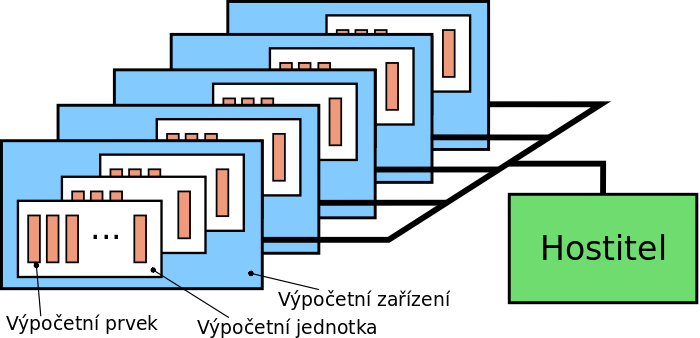
\includegraphics{fig/opencl_platform_model_cl}
	}
    \end{center}
    \caption{Model OpenCL platformy \cite{Khronos:2015}}
    \label{platform}
\end{figure}
\subsubsection{Model provádění}
Jak již bylo zmíněno aplikace se dělí na dvě části: OpenCL kernel a hostitelskou aplikaci.
Hostitelská aplikace provádí inicializaci a řízení chodu kernelu, zatímco kernel provádí samotný
výpočet. Výpočty jsou prováděny na pracovních položkách ({\it work-item}) jenž můžeme sdružovat do
pracovních skupin ({\it work-group}).

 Hostitel má za úkol spravovat kontext aplikace a~na jeho základě nastavit prostředí, ve
kterém bude kernel provádět operace. V~prostředí musíme specifikovat a~nastavit tyto položky:
\begin{itemize}
    \item Zařízení -- jedno a~více zařízení ovladatelných platformou OpenCL.
    \item Objekty kernelu -- OpenCL funkce s~přednastavenými argumenty podle vybraného
        zařízení.
    \item Objekty programu -- zdrojový kód a~jeho spustitelná verze, které implementují
        kernely.
    \item Objekty paměti -- proměnné, ke kterým může přistupovat hostitel i~OpenCL zařízení.
	Instance kernelů během svého provádění operují s~těmito objekty.
\end{itemize}
Hostitel se zařízením komunikuje pomocí front příkazů, do nichž se příkazy rozřadí podle
typu operace. Jednotlivé příkazy ve frontě se provádí relativně k~ostatním příkazům. Pořadí
provádění může být definováno následujícími modely:
\begin{itemize}
    \item {\it In-order} -- příkazy se provádí a~mají efekt tak, jak do fronty přišly.
    \item {\it Out-of-order} -- pořadí provedení příkazů je omezeno pouze explicitně uvedenými
        synchronizačními body nebo explicitně definovanými závislostmi na událostech.
\end{itemize}

\subsubsection{Model paměti}
Práce s~pamětí v~OpenCL se značně liší od klasického přístupu, který známe ze standardních
aplikací určených pro běh pouze na CPU. Paměťový model OpenCL popisuje obsah, strukturu a~chování
paměti používané v~platformě vytvořené tímto frameworkem.

 Pro každou aplikaci je třeba přesně definovat, jak přesně bude její paměť vypadat.
Model dělíme na čtyři části:
\begin{itemize}
    \item {\it Oblasti paměti} -- definuje, se kterými oblastmi paměti hostitel a~zařízení ve
	stejném kontextu mohou pracovat.
    \item {\it Objekty paměti} -- jsou definované v~OpenCL API, o~správu se stará hostitel i
	zařízení.
    \item {\it Sdílenou virtuální paměť} -- tvořící virtuální adresový prostor přístupný oběma
	částem aplikace.
    \item {\it Model konzistence} -- definuje pravidla pro oblasti paměti, které jsou používané
	více jednotkami naráz a~zaručuje, že je dodrženo pořadí operací s~pamětí a~že jsou data po
	celou dobu validní. Taktéž definuje synchronizaci nad těmito oblastmi.
\end{itemize}
Pro nás je nejdůležitější pochopit, jak je paměť strukturována a~jak na sebe navazují
jednotlivé oblasti. To je nejlépe patrné z~obrázku \ref{memory}. Paměť je rozdělena do následujících
částí:
\begin{itemize}
    \item paměť hostitele (RAM apod.),
    \item paměť zařízení,
    \begin{itemize}
	\item {\it globální paměť} -- oblast přístupná pro čtení i~zápis všem jednotkám
	    v~kontextu nezávisle na zařízení,
	\item {\it paměť konstant} -- před zahájením výpočtu alokovaná a~inicializována
	    hostitelem a~v~průběhu výpočtu neměnná oblast,
	\item {\it lokální paměť} -- oblast přístupná všem pracovním položkám ve stejné pracovní
	    skupině,
	\item {\it soukromá paměť} -- oblast přístupná pouze jedné pracovní položce.
    \end{itemize}
\end{itemize}
\begin{figure}[ht]
    \begin{center}
	\scalebox{0.3}{
	    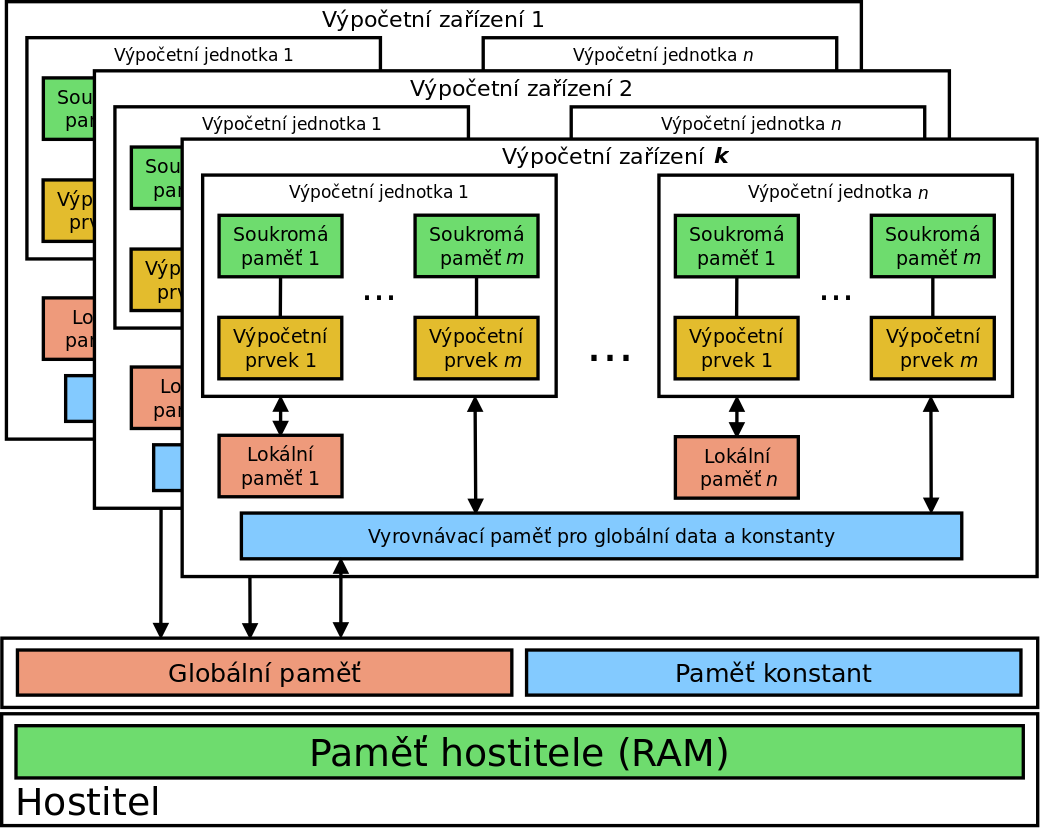
\includegraphics{fig/opencl_memory_structure_cl}
	}
    \end{center}
    \caption{Struktura paměti OpenCL \cite{Khronos:2015}}
    \label{memory}
\end{figure}
\subsubsection{Programovací model}
Tento model lze také nazvat jako OpenCL framework. Framework se skládá ze třech komponentů. Zde za
zmínku stojí OpenCL kompilátor. Ten podporuje pokročilý jazyk SPIR-V a~jazyk OpenCL C. Další
jazyky mohou být podporovány některými implementacemi kompilátoru.


\chapter{Nástroj Wrathion}
\label{ch:wrathion}
Jedná se o~nástroj vytvořený Janem Shmiedem v~roce 2014 v~rámci jeho diplomové
práce~\cite{Schmied}. Nástroj byl vytvořen pro použití v~projektu {\it Moderní prostředky pro 
boj s~kybernetickou kriminalitou na Internetu nové generace, MV, VG20102015022}.
\section{Hlavní části Wrathionu}
Nástroj slouží ke obnovování hesel pomocí brute-force útoků na tato hesla. Skládá se ze tří
částí:
\begin{itemize}
	\item jádra -- zprostředkovávajícího funkcionalitu potřebnou pro crackování,
	\item modulů -- skrze které je zajištěna podpora crackování různých formátů,
	\item aplikace -- umožňující pracovat s~frameworkem a~moduly pomocí CLI rozhraní.
\end{itemize}
\begin{figure}[ht]
    \begin{center}
	\scalebox{0.34}{
	    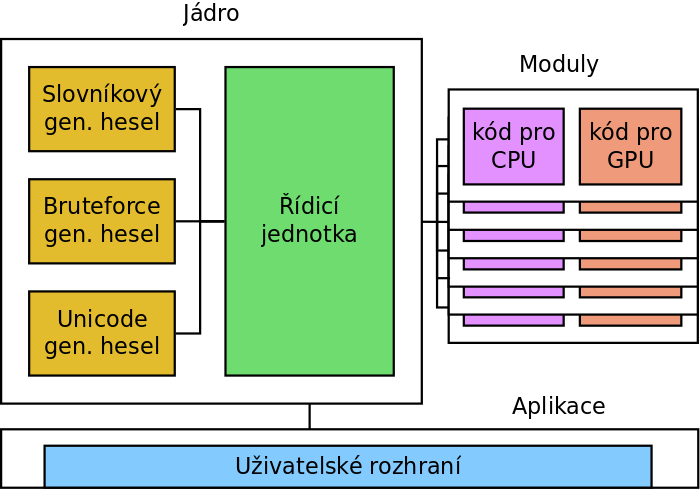
\includegraphics{fig/wrathion_structure_cl}
	}
    \end{center}
    \caption{Schéma struktury nástroje Wrathion \cite{Hranicky}}
    \label{memory}
\end{figure}
\subsection{Generátory hesel}
První částí Wrathionu jsou generátory hesel pro útoky. Jedná se o~esenciální
funkcionalitu. Bez generátoru hesel není možné útoky provádět. V~nástroji jsou momentálně
implementovány tyto typy generátorů~\cite{Hranicky}:
\begin{itemize}
    \item {\it Brute-force} -- postupně generuje všechny možné permutace ze zadaných znaků.
    \item {\it Unicode} -- jedná se o~upravený brute-force generátor. V~tomto případě je nastavena
	vstupní abeceda na všechny Unicode znaky a~z~nich jsou generovány možné permutace hesel.
    \item {\it Rule-based} -- velmi podobný předchozím variantám ovšem umožňuje specifikovat různá
	podpůrná pravidla pro generování hesel. Například, že má být první písmeno velké, druhé má
	být 'a' a~že poslední 2 znaky jsou číslice. Toto umožňuje zúžení počtu permutací a~tedy
	snižuje čas potřebný k~vygenerování všech jejich variant (tento typ generátoru je teprve
	ve vývoji).
    \item {\it Dictionary} -- slovníkový generátor, který využívá externí soubory s~často
	používanými hesly.
\end{itemize}
Nejčastěji používaným generátorem je brute-force, který je ovšem výpočetně náročný. Jedná se
však o~snadno paralelizovatelný generátor, proto je příhodně implementován i~jako kernel běžící na
GPU.
\subsection{Crackery}
Pojem {\textit cracker} v kontextu wrathionu vyjadřuje část programu provádějící kroky potřebné k
ověření, zda vygenerované heslo je shodné s heslem, které bylo použito pro šifrování. Při použití
akcelerace obnovy hesel na GPU je crackrem OpenCL kernel.
Druhou částí jsou samotné crackery, které dělíme podle toho, kdo provádí generování hesel a
kdo provádí porovnávání hesel:
\subsubsection{CPU cracker}
Zde se standardně spustí již předkompilovaný cracker napsaný v~C++ (viz. Obrázek \ref{CPU}). Není
zde žádný větší problém s~generováním ani následným ověřováním hesel, ovšem výpočetní síla
u~paralelizovatelných algoritmů není na CPU ani zdaleka tak vysoká jako na GPU. Proto, pokud je to
možné, volíme druhou variantu crackeru.
\begin{figure}[ht]
    \begin{center}
	\scalebox{0.3}{
	    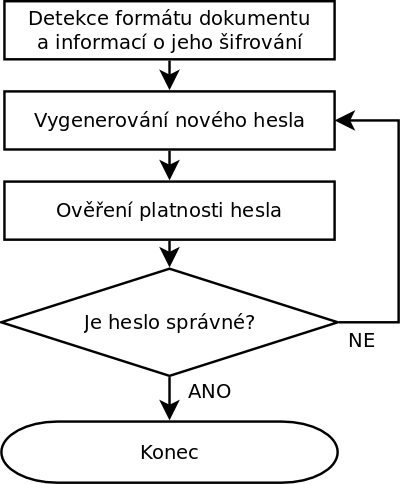
\includegraphics{fig/proces}
	}
    \end{center}
    \caption{Proces generování a~ověřování hesel na CPU \cite{Schmied}}
    \label{CPU}
\end{figure}

\subsubsection{GPU cracker}
Cracker může pracovat ve dvou režimech (viz. Obrázek \ref{CPUGPU}). V~prvním hesla generujeme na
CPU a~pak je posíláme do paměti GPU, kde jsou crackerem zpracována. To má ovšem velkou nevýhodu
v~tom, že musíme pořád posílat data z~paměti hostitele (CPU) do privátní paměti výpočetního prvku
(výpočetní jednotka na GPU).
\begin{figure}[ht]
    \begin{center}
	\scalebox{0.32}{
	    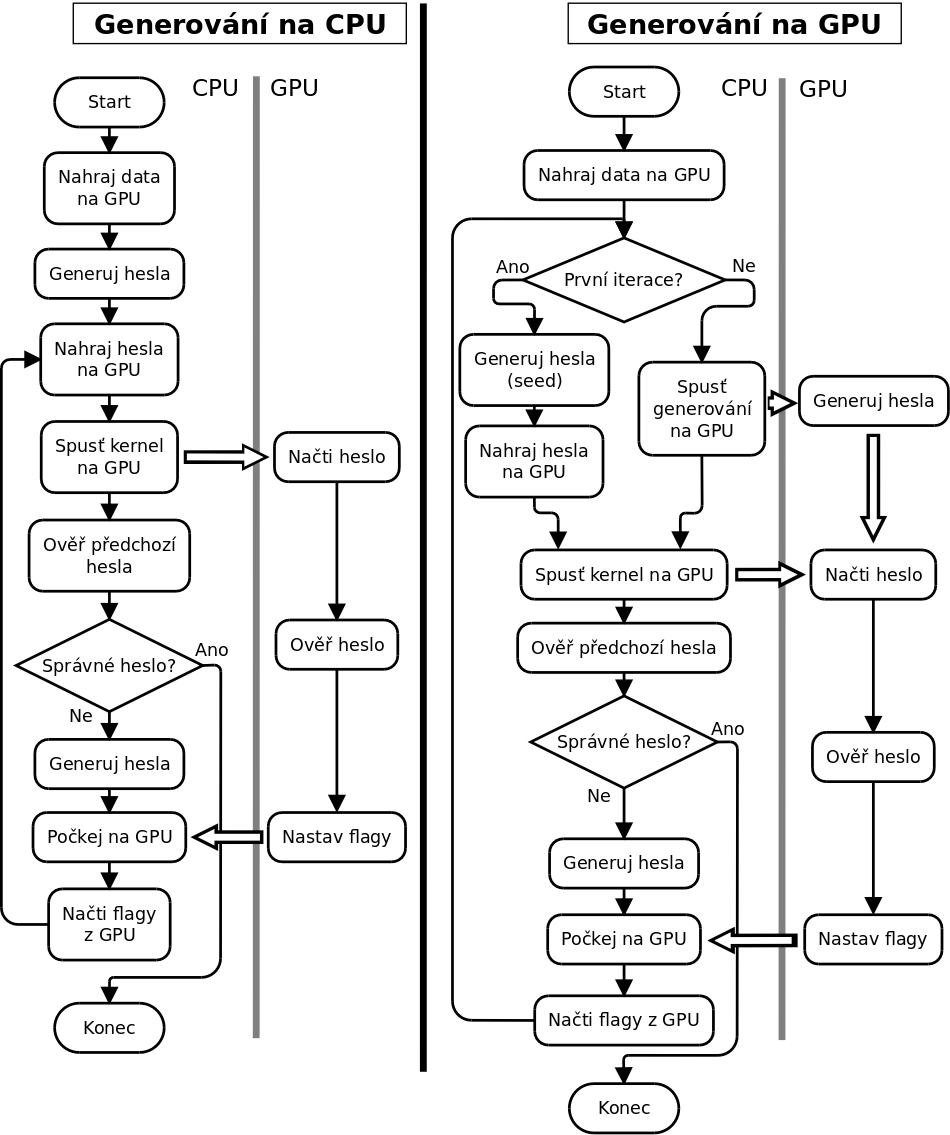
\includegraphics{fig/generators}
	}
    \end{center}
    \caption{Proces generování hesel na CPU a~ověřování na GPU \cite{Schmied}}
    \label{CPUGPU}
\end{figure}

 Druhou a~efektivnější možností je generovat hesla přímo na GPU do privátních pamětí čím
minimalizujeme množství dat, které musí putovat od hostitele k~zařízení. Tímto snížíme výslednou
prodlevu výpočtů.

 V~obou případech je nutné před zahájením jakýchkoliv operací GPU
 inicializovat\linebreak OpenCL systém. Tedy vytvořit kontext, fronty příkazů, zajistit načtení a
 přeložení požadovaného kernelu a~až poté nahrát nebo vygenerovat data do/na GPU.

\subsection{Moduly}
Nástroj je navržen s~velkým důrazem na modularitu. V~současné době obsahuje pouze tři moduly.
Další moduly pro Wrathion jsou ve fázi vývoje~\cite{Hranicky}.

\subsubsection{Modul ZIP}
ZIP modul v~původním návrhu obsahuje pouze šifrování obnovování hesel z~archivů šifrovaných
algoritmy PKZIP, AES-128, AES-192, AES-256, což zanechává prostor pro implementaci dalších, formátem
{\it .ZIP}, podporovaných metod. Zajímavostí je, že tento modul byl schopný v~době svého vzniku
obnovit heslo šifrovaných {\it .DOCX} souborů, avšak tento nedostatek u~zabezpečení formátu {\it
.DOCX} byl později odstraněn a~tento modul již tedy není schopen obnovit heslo u~souborů vytvořených
po zmíněné aktualizaci.

\subsubsection{Modul DOC}
Další modul pracuje s~formátem {\it .DOC}, který byl pokládán za základní formát aplikace MS Word
z~balíku MS Office. Tento formát byl s~příchodem MS Office 2007 nahrazen formátem {\it .DOCX}.
Nástroj ve své původní podobě obsahuje pouze podporu pro {\it .DOC} formát. Tvorba modulů pro
novější formát {\it .DOCX} spolu s~formáty používanými v~jiných aplikacích balíku MS Office je ve
fázi vývoje.

\subsubsection{Modul PDF}
Prozatím poslední vytvořený modul pracuje s~formátem {\it .PDF}. Zde jsou již implementovány
bezpečnostní revize 1-5. Nástroj počítá i~s~implementací revize 6. Vývoj této funkcionality může
být započat až po zveřejnění specifikace této revize.


\chapter{Analýza formátů .ZIP a~.7z}
\label{ch:formaty}
\section{Formát .ZIP}
Jedná se o~jeden z~prvních formátů souborových archivů, který podporoval kompresi dat. V~roce 1989
vytvořil Phil Katz program PKZIP v~rámci něhož byl představen nový formát .ZIP. Specifikace
formátu .ZIP byla publikována pod veřejnou doménou. Tímto krokem pomohl formátu se stát
celosvětovým otevřeným standardem~\cite{PKWARE:2015}. V~roce 2015 byl formát, ve své specifikaci
6.3.3 z~roku 2012, přijat Mezinárodní organizací pro normalizaci (ISO) a~Mezinárodní
elektrotechnickou komisí (IEC) jakožto standard definovaný dokumentem ISO/IEC
21320-1:2015~\cite{ISOIEC:2015}.

 Formát podporuje velké množství různých komprimačních algoritmů: Store (bez komprese),
UnShrinking, Expanding, Imploding, Tokenizing, Deflating, Enhanced Deflating, BZIP2, LZMA, WavPack
a PPMd~\cite{PKWARE:2014}. 

 Obdobně je to i~s~podporou různých šifrovacích algoritmů:
\begin{itemize}
    \item {\it PKWARE šifrování} -- prvotní šifrování,
    \item {\it DES, 3DES(112-bit a~168-bit)} -- podporováno od verze 5.0 z~roku 2002,
    \item {\it RC2 (40-bit, 64-bit a~168-bit)} -- podporováno od verze 5.0 z~roku 2002,
    \item {\it RC4 (40-bit, 64-bit a~168-bit)} -- podporováno od verze 5.0 z~roku 2002,
    \item {\it AES (128-bit, 192-bit a~256-bit)} -- podporováno od verze 5.2 z~roku 2003.
\end{itemize}
V současnosti žádný z~volně dostupných, ani komerčních nástrojů neumožňuje vytvoření archivů se
šifrováním DES, RC2 a~RC4. Z~toho tedy plyne, že pravděpodobnost výskytu archivů šifrovaných těmito
metodami je minimální, a proto se jimi tato práce nebude dále zabývat.

\subsection{Struktura souboru}
\label{ssec:zip_struct}
Archivy jsou soubory obsahující další soubory. Je možné je tedy považovat za \uv{schránky}, do nichž
lze vkládat, ale i~vybírat, určité soubory různých typů. U~formátu .ZIP lze do archivů navíc ukládat
i~adresáře a~tak ukládat celé struktury tvořené z~adresářů a~souborů (viz. Obrázek~\ref{zipstruct}).

\begin{figure}[ht]
    \begin{center}
	\scalebox{0.225}{
	    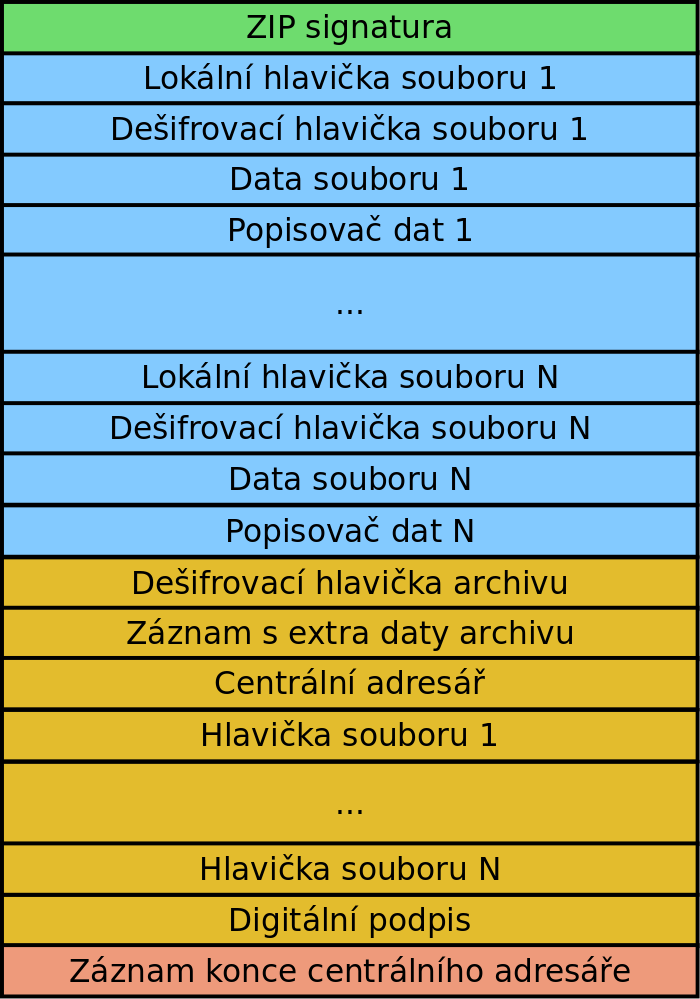
\includegraphics{fig/zip_structure_cl}
	}
    \end{center}
    \caption{Struktura .ZIP souboru \cite{PKWARE:2014}}
    \label{zipstruct}
\end{figure}

 Obsah souboru archivu lze pro lepší orientaci rozdělit na část obsahující definice a~data
uložených souborů a~na část reprezentující organizaci adresářů a~souborů.
\begin{itemize}
    \item První část obsahuje záznamy, jenž se opakují pro každý uložený soubor. Jeden takovýto
záznam musí obsahovat alespoň lokální hlavičku souboru a~data souboru. Pokud je nastaven
3. bit položky {\it General purpose bit flag} v~lokální hlavičce souboru, musíme ještě počítat
s~tím, že za data byla přidána sekce {\it Data description} o~velikosti 12 bajtů.
    \item Druhá část se skládá ze struktury hlaviček centrálního adresáře (Central Directory
	Header). Počet těchto hlaviček odpovídá počtu adresářů a~souborů obsažených v~tomto
	archivu. Hlavička centrálního adresáře začíná signaturou [0x50, 0x4b, 0x01, 0x02], podle které je
	v~souboru identifikovatelný začátek hlavičky. Za ní následují metadata souboru, např.: datum a~čas
	poslední úpravy obsaženého souboru, velikost před a~po kompresi atd. Tato struktura hlaviček je
	ukončena položkou {\textit Záznam konce centrálního adresáře}. Ten začíná signaturou [0x50, 0x4b, 0x05, 0x06]
	a~obsahuje informace o~tom na kterém disku je soubor uložen, na kterém disku začíná struktura
	centrálního adresáře a~další.
\end{itemize}
Od verze formátu 6.2 jsou před hlavičkou centrálního adresáře další položky, a~to hlavička
pro dešifrování archivu a~záznam o~extra datech archivu. Tyto položky byly přidány
v~souvislosti s novou funkcí pro šifrování obsahu hlaviček centrálního adresáře.

\subsubsection{Řídící struktury definující šifrování}
 Dosud byla popisována pouze základní struktura archivu. Nás ale především zajímají struktury
archivů, jež obsahují soubory v~zašifrované podobě. Zda je soubor šifrován, lze zjistit z~jeho
lokální hlavičky nebo z~jeho hlavičky centrálního adresáře, konkrétně z~prvního a~sedmého bitu
položky {\it General Purpose Bit Flag}. Nastavení prvního bitu indikuje, že je soubor šifrován.
\begin{itemize}
    \item Pokud platí, že není zároveň nastaven i~sedmý bit, je za lokální hlavičku souboru
        přidána hlavička šifrování. Hlavička šifrování se váže pouze k~šifrování pomocí tradiční
        metody od společnosti PKWARE.
    \item Pokud je nastaven i~sedmý bit indikující použití takzvaného \uv{silného
	šifrování}, hlavička šifrování se negeneruje, ale přidávají se informace o~šifrování do
        hlavičky centrálního adresáře a~generuje se záznam s~hlavičkou pro dešifrování, jehož
	část se tváří jako součást dat souboru a~nachází se na samém počátku šifrovaných dat
	souboru.
\end{itemize}
Informace o~metodě šifrování, délce klíče atd., jsou z~důvodů vyšší bezpečnosti uvedeny v~druhé
části souboru v~položce {\it Extra Fields} v~hlavičce centrálního adresáře příslušící souboru.
Položku {\it Extra Fields} poznáme podle signatury [0x00, 0x17]. Další položky obsahují informace
o~použitém šifrovacím algoritmu, délce klíče pro šifrování a~pole příznaků {\it Flags} definující,
zda je archiv šifrovaný, jaká je použita kompresní metoda, co je vyžadováno pro dešifrování. Tedy
zda je možná provést dešifrování pouze pomocí hesla nebo certifikátu anebo je-li možné použít
oboje. Další možnosti závisí na použitém certifikátu.

 Záznam pro dešifrování obsahuje inicializační vektor (IV), identifikátor algoritmu pro
dešifrování, bitovou délku šifrovacího klíče, zašifrovaný vzorek náhodných dat (Erddata), a~hlavně
o~informace pro validaci hesla (VData) a~kontrolní součet CRC-32 (VCRC32)\footnote{{\it Cyclic Redundancy Code} -
speciální hešovací funkce sloužící pro detekci chyb / změn dat oproti původní hodnotě} těchto
validačních dat. 

\section{Formát .7z}
\label{sec:7z}
Vznik tohoto formátu se datuje do roku 1999 a~jeho autorem je Igor Pavlov. Stejně jako aplikace
7-Zip a~nástrojů spojených s~tímto formátem (7-Max, 7-Benchamark). Formát taktéž slouží
k~vytvoření souborových archivů podobně jako .ZIP. Formát se proslavil hlavně svojí otevřeností a
modulární strukturou. Ta umožňuje skládání libovolných kompresních, konverzních a~šifrovacích
metod~\cite{7z:2015}.

 Mezi podporované kompresní metody se řadí LZMA, LZMA2, PPMD, BCJ, BCJ2, BZip2 a
Deflate. Jako výchozí metoda je brána LZMA. Hlavní výhody této metody jsou:
\begin{itemize}
    \item vysoký kompresní koeficient,
    \item proměnná velikost slovníku,
    \item malé nároky na paměť při dekompresi,
    \item podpora zpracování pomocí multi-threading a~hyper-threading.
\end{itemize}
Další výhodou formátu je podpora komprese velkých souborů, názvy souborů v~Unicode
kódování, možnost spojení více souborů do jednoho toku, který je pak teprve komprimován, komprese
a šifrování hlaviček archivů a~další.

 Standardně použitou šifrovací metodou je AES-256 vyžadující 256-bitové šifrovací heslo.
Takovéto heslo se vytváří pomocí hešovací funkce SHA-256 z~uživatelem zadaného hesla. Pro ještě
vyšší zabezpečení je provedeno \(2^{19}\) iterací při každém vytváření hesla. To může mít na
slabších zařízeních za následek znatelnou prodlevu, než začne komprese souborů a~šifrování.

\subsection{Struktura souboru}
\label{ssec:7z_struct}
Neprázdný soubor tohoto formátu má čtyři části, které v~něm musí být obsaženy (viz. Obrázek
\ref{7zstruct}). Jedná se o~položky: 
\begin{itemize}
    \item Na začátku souboru se nachází hlavička. Jedná se o~hlavičku {\it 7zSignature} se
	signaturou ['7', 'z', 0xBC, 0xAF, 0x27, 0x1C] definující začátek souboru daného typu.
	Za ní v~rámci stejné hlavičky jsou informace o~verzi archivu, CRC hlavičky a položky
	specifikující pozici následující hlavičky. Najdeme zde relativní adresu (uvedena jako
	vzdálenost od konce úvodní hlavičky), následuje pak délka další hlavičky a~CRC pro tyto dvě
	položky.
    \item Druhá část obsahuje zpracovaná data vytvořených proudů, tedy data samostatných nebo
	případně i~spojených souborů po kompresi, šifrování apod.
    \item Třetí část obsahuje zpracované informace sloužící jako podpůrná data pro hlavičku a~její
	položky.
    \item Poslední čtvrtá částí je 7z hlavička ({\it 7zHeader}), jejíž začátek je definován
	v~úvodní hlavičce. Tato hlavička má proměnnou délku a~strukturu. Je ji tedy potřeba
	procházet postupně a~zjišťovat, které položky jsou přítomny a~které ne. K~identifikaci
	jednotlivých položek slouží jednobajtový identifikátor. Identifikátory jsou v rozmezí 0x00
	až 0x19. Máme tedy k~dispozici 25 položek s~různou velikostí, strukturou a~položkami.
	Jedinými povinnými údaji v~hlavičce jsou položky značící začátek hlavičky (0x01) a~konec
	hlavičky (0x00). Všechny ostatní položky jsou případně umístěny mezi ně a~začínají
	příslušným identifikátorem~\cite{Pavlov:2010}. 
\end{itemize}
\begin{figure}[ht]
    \begin{center}
	\scalebox{0.35}{
	    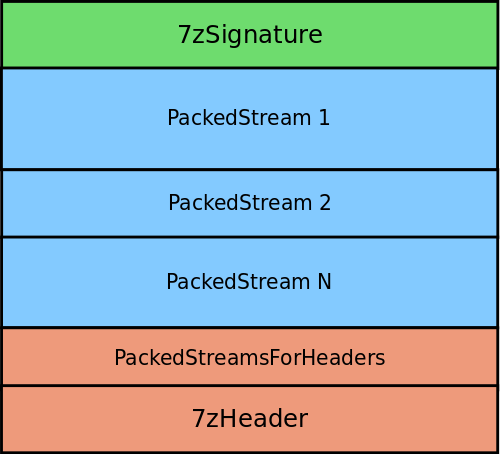
\includegraphics{fig/7z_structure_cl}
	}
    \end{center}
    \caption{Struktura .7z souboru \cite{Pavlov:2015}}
    \label{7zstruct}
\end{figure}
Pro účely této práce nás především zajímá hlavička {\it 7zHeader} a~v~ní obsahy položek nesoucích
informace o~proudech dat (0x03 nebo 0x04). V~nich konkrétně položka informace o~kodérech (0x07),
ve které se musíme propracovat k~poli bajtů {\it CodecInfo}. Hodnoty tohoto pole musíme otestovat
a zjistit, zda se shodují s~identifikátorem standardní šifrovací metody AES-256 + SHA-256
[0x06, 0xF1, 0x07, 0x01]~\cite{Pavlov:2015}. Zde je třeba také nalézt data o~použité kompresi.
Kompresní metoda LZMA má identifikátor [0x03, 0x01, 0x01]. Další důležitou položkou pro ověření
hesla je CRC šifrovaného souboru.

Tento typ archivu bohužel neobsahuje žádnou jinou metodu ověření hesla než pomocí spočítání a
porovnání CRC hodnot. K~tomu je nutné nejprve celý soubor dešifrovat a dekomprimovat, což přidává
na náročnosti celého ověřovacího procesu.

\section{Srovnání}
Pokud budeme srovnávat formáty z~pohledu komprese, zjistíme, že .7z je dle
měření\footnote{\url{http://www.howtogeek.com/200698/benchmarked-whats-the-best-file-compression-format/}}
efektivnější než .ZIP. Z pohledu této práce nás spíše zajímájí valstnosti týkající se zabezpečení.

 Šifrování formátu .ZIP metodou PKZIP nemá smysl ani porovnávat s~ostatními, neboť se jedná
o~metodu, která již nevyhovuje dnešním bezpečnostním standardům~\cite{PKWARE:2014}. 

 Pokud se však podíváme na silnější metody zabezpečení, zjistíme, že formáty jsou z~hlediska
bezpečnosti vyrovnané. Oba dva podporují AES-256 s~využitím nějaké hešovací metody pro zabezpečení
hesla. Oba formáty také podporují šifrování hlaviček obsahujících informace o~metodách, které jsou
používány a~jaké soubory obsahují.

 Formát .ZIP překonává .7z možností použití elektronických podpisů (certifikát typu X.509v3)
k~šifrování souborů namísto hesel. 7z tuto funkcionalitu vůbec neobsahuje. 



\chapter{Návrh modulů}
\label{ch:moduly}
Tato kapitola vysvětluje, jak lze z~výše popsaných algoritmů, technologií a~strukturálních
analýz archivů vytvořit rozšiřující moduly pro nástroj Wrathion. Cílem je obecně popsat, průchod
souboru jednotlivých formátů. Tedy jaká data se z~nich je potřeba získat, jaké operace je
potřeba provést nad vygenerovanými hesly a~jaké kroky je nutné provést při ověřování shody hesel.

\section{Modul ZIP}
Protože nástroj Wrathion modul ZIP již obsahuje, nemusíme zde řešit návrh celého modulu, ale pouze
rozšíření jeho funkcionality o~zatím nepodporované metody zabezpečení.

 Momentální verze ZIP modulu podporuje pouze staré šifrování PKWARE a~šifrování WinZip AES. Podpora
šifrování AES je tedy neúplná. Modul momentálně podporuje pouze speciální verzi AES, jež si
vytvořili vývojáři nástroje WinZip. Tato verze uvažuje vlastní ořezanou AES hlavičku a~vytvoření
nové metody zapsané do příznaků souboru. Existují ovšem nástroje jako SecureZIP od firmy PKWARE umožňující také
zašifrovat obsah archivů pomocí šifrovací metody AES, kterou současný modul, i~přes podporu zjištění
hesla pro při použití šifrování AES, nepodporuje.

% Další šifrovací metodou, kterou nabízí nástroj SecureZIP je 3DES, kterou momentální verze
%nepodporuje vůbec a~je tedy nutné tuto funkcionalitu doplnit.

\subsection{Zjištění informací z~archivu}
Z archivu musíme získat informace nutné pro rozhodnutí, zda se jedná o~ZIP soubor, zda je soubor
šifrován, jakou metodou je šifrován, jaké jsou inicializační hodnoty použité při šifrování apod. To
vše je potřeba pro rozšíření funkcionality modulu. Postup získání informací se nesoustředí na
získání informací nutných pro ověření hesla u již implementovaných metodách, ale pouze informací
důležitých pro rozšíření funkcionality modulu (detailní popis hlaviček a~hodnot v~nich je
v~sekci~\ref{ssec:zip_struct}):
\begin{enumerate}
    \item Zjištění signatury -- podíváme se na první 4 bajty a~porovnáme je se signaturou [0x50,
	0x4B, 0x03, 0x04]. Tím ověříme, zda se jedná o~ZIP soubor.
    \item Přečtení {\it General purpose bit flag} -- hodnotu příznaků získáme z~lokální hlavičky
	prvního souboru.
    \item Analýza příznaků -- zjišťujeme zda jsou nastaveny první a~sedmý bit příznaků na hodnotu
	1. Pokud nalezneme šifrování u~jednoho souboru předpokládáme, že všechny ostatní soubory
	jsou taktéž šifrované a~že byla použita stejná šifrovací metoda. Pokud je nastaven i~13.
	bit musíme provést čtení dešifrovací hlavičky archivu a~pomocí ní dešifrovat celou
	strukturu centrálního adresáře. Postup dešifrování je identický s~dešifrováním souborů.
    \item Přečtení {\it Compression method} -- z~některé z~hlaviček %\footnotemark[\value{footnote}] 
	souboru. Tato položka nás zajímá, pouze pokud byly bity jedna a~sedm příznaků nastaveny na
	hodnotu 1. Číslo uvedené v~této položce nám dovoluje zjistit, zda byla použita šifrovací
	metoda WinZip AES (hodnota 99). Použití jiné hodnoty indikuje použití některé z~dalších
	šifrovacích metod definovaných ve specifikaci formátu .ZIP~\cite{PKWARE:2014}.
    \item Přečtení {\it Extra fields} -- potřebujeme najít hlavičku s~daty o~šifrování, která se
	může vyskytnout pouze za hlavičkou souboru v~centrálním adresáři. V~tomto kroku zjistíme
	informace o~použité šifrovací metodě, délce klíče atd.
    \item Získání hodnot hlavičky pro dešifrování -- nachází se před uloženými daty souboru.
	Potřebujeme získat použitá inicializační data potřebná pro šifrovací s~dešifrovací funkce.
	A~také data pro ověření hesla včetně jejich kontrolního součtu (CRC32).
\end{enumerate}

\subsection{Obnova hesel}
Jakmile takto získáme všechna potřebná data, přesuneme se k~hledání použitého hesla. Tento proces
bude možné realizovat za využití CPU nebo GPU. Pro obě tato zařízení je nutné vytvořit samostatný
kód. Kód pro CPU čistě v~jazyce C++ s~možností využití některých již implementovaných funkcí a
generátorů obsažených v~nástroji Wrathion. Pro GPU je třeba vytvořit kód v~C++, který poběží na
CPU, bude inicializovat GPU a~rozdělovat práci pracovním jednotkám na ní umístěných a~poté kernel
v~OpenCL pro implementování kernelu, který poběží na pracovních jednotkách. Avšak v~obou
případech půjde o~totožný Algoritmus~\ref{alg:zip_ver}.

\begin{algorithm}[ht]
    \SetStartEndCondition{ (}{)}{)}\SetAlgoBlockMarkers{}{}%
    \SetKwFor{For}{for}{\string:}{}%
    \SetKwIF{If}{ElseIf}{Else}{if}{}{else if}{else}{}%
    \SetKwRepeat{Repeat}{repeat}{until}%
    \SetKwInOut{Input}{vstup}\SetKwInOut{Output}{výstup}
    \AlgoDisplayBlockMarkers\SetAlgoNoLine%
    \DontPrintSemicolon
    \Input{Data získaná z~hlavičky pro dešifrování (IV, Erd, Dlen, Data)}
    \Output{Poslední vygenerované heslo}
    \Repeat{$ CRC \neq spocitejCRC32 (Data, Dlen-4) $}{
	heslo = generujHeslo()\;
	odvozene\_heslo = odvodHeslo (SHA1(heslo))\;
	rd = desifruj (Erd, odvozene\_heslo, IV)\tcc*{Random hodnota pro šifrování}
	odvozene\_heslo = odvodHeslo (SHA1(rd + IV))\;
	desifrovana\_data = desifruj (Data, odvozene\_heslo, IV)\;
	CRC = *(uint32*)(\&Data[Dlen-4])\tcc*{Poslední 4 bajty jsou CRC}
    }
    \Return heslo\;
    \caption{Princip ověření hesla u ZIP archivu}\label{alg:zip_ver}
\end{algorithm}

\section{Modul SevenZ}
V~tomto případě se jedná o~úplně nový modul. Bude tedy potřeba nadefinovat všechny struktury
potřebné k~provozu modulu v~rámci nástroje Wrathion a~implementovat metody šifrování, hešování,
odvozování hesel a~jiné používané formátem .7z.

\subsection{Zjištění informací z~archivu}
Archiv formátu .7z v~sobě, stejně tak jako .ZIP archiv, nese informace nutné pro umožnění
dešifrování souboru. V~tomto případě je však o~něco složitější je získat. Struktura 7z archivu
je hodně komplexní a~proměnlivá. Struktura hlaviček do značné míry připomíná databázi. Pro
detailní porozumění struktuře řídících dat formátu je třeba nahlédnout do souboru
7zFormat.txt~\cite{Pavlov:2010}. Potřebné informace lze získat následujícím 
teoretickým postupem:
\begin{enumerate}
    \item Ověříme signaturu -- prvních 6 bajtů souboru se musí rovnat hodnotě ze~sekce \ref{ssec:7z_struct}. 
    \item Přejdeme na pozici 6 bajtů za signaturou, kde	prvních 8 bajtů obsahuje pozici hlavičky.
	Na dalších 8 bajtech je délka hlavičky.
    \item Přejdeme na začátek hlavičky.
    \item Přejdeme na záznam se signaturou 0x06 nesoucí pozici dat, k~níž přičteme 32.
    \item Přejdeme na záznam se signaturou 0x09 nesoucí délku proudu dat.
    \item Přejdeme na záznam se signaturou 0x0B, ve které hledáme hodnoty [0x06, 0xF1, 0x07, 0x01]
	a [0x03, 0x01, 0x01] značící 7zAES a LZMA. Zde hledáme inicializační vektor, počet iterací použití SHA256 (implicitně
	19) pro 7zAES a inicializační data slovníků pro LZMA.
    \item Přejdeme na záznam se signaturou 0x0A, ze kterého získáme CRC dat souboru.
\end{enumerate}

\subsection{Obnova hesel}
Jakmile tato data získáme, můžeme se přesunout k~hledání hesla. Tento proces, popsány
Algoritmem~\ref{alg:7z_desifr}, lze plně realizovat pouze na CPU. Formát 7z totiž může obsahovat
soubory o~velké velikosti, které by se nemusely vejít do paměti GPU. Musíme zde vzít totiž
v~potaz, že potřebujeme mít v~paměti prostor o~velikosti souboru pro každou výpočetní jednotku GPU,
na které poběží kernel. Řešení tohoto problému je popsáno v~sekci \ref{ssec:7zcrackercpu}.

\begin{algorithm}[!h]
    \SetStartEndCondition{ (}{)}{)}\SetAlgoBlockMarkers{}{}%
    \SetKwFor{For}{for}{\string:}{}%
    \SetKwInOut{Input}{vstup}\SetKwInOut{Output}{výstup}
    \SetKwRepeat{Repeat}{repeat}{until}%
    \AlgoDisplayBlockMarkers\SetAlgoNoLine%
    \DontPrintSemicolon
    \Input{Data získaná z~hlaviček (IV, iteraci, lzma\_data)}
    \Output{Poslední vygenerované heslo}
    \Repeat{$ CRC \neq spocitejCRC32 (data) $}{
	heslo = generujHeslo()\;
	klic = derivuj\_heslo(heslo, iteraci)\;
	desif\_data = desifruj\_data(klic, IV, sif\_data)\;
	data = dekomprimuj(desif\_data, lzma\_data)\;
    }
    \Return heslo\;
    \caption{Princip ověření hesla archivu 7z}
    \label{alg:7z_desifr}
\end{algorithm}
    
\chapter{Implementace}
\label{ch:implementace}
Tato kapitola se věnuje popisu implementace přidané funkcionality modulu ZIP a nového modulu pro
7z do nástroje Wrathion. Jsou v~ní také zmíněny použité knihovny implementující dešifrovací a
dekomprimační metody společně s jejich verzemi. Kapitola je rozdělena do dvou částí, každá
reprezentující jeden z~formátů, jimiž se tato práce zabývá.

\section{Implementace modulu ZIP}
Jak již bylo zmíněno, tento modul bylo třeba pouze doplnit o~další funkcionality týkající se 
především podpory metod šifrování. Konktrétně se jednalo o~metody šifrování souborů AES a DES a také
o~metodu umožňující šifrování {\textit Central Directory} záznamu. Tyto metody jsou definované ve
standardu formátu ZIP vydaném firmou PKWARE v~rámci APPNOTE.txt a používány
v~nástrojích z~rodiny SecureZIP od PKWARE.

\subsection{ZIPFormat}
Tato třída slouží ke čtení potřebných informací z~archívu na vstupu. Získává tedy imformace o~tom
jaká šifrovací metoda byla použita na základě čehož pak hledá další pro nás důležitá data ve
struktuře souboru. Data jsou ukládána do struktury $ZIPInitData$, která je použita pro
inicializaci nových instancí tříd crackerů. 

 Třída byla upravena tak, aby byla schopna detekovat výše zmíněné metody a uložit data potřebná pro
následné ověřování hesel.

\subsection{ZIPStAESCrackerCPU}
Jedná se o~třídu s~implementací pro ověření hesla metodou AES čistě na CPU. Třída obsahuje funkci
pro ověření hesla $checkPassword()$ a funkce $derive()$, $derive\_key()$ a $sha1()$ pro vytvoření
šifrovacích klíčů.

Třída využívá implementace šifrovací funkce AES použité v~nástroji
UnRAR\footnote{\url{http://www.rarlab.com/rar\_add.htm}}, kde je implementována jako třída Rijndael
pod licencí Public Domain. Datové typy použité v~převzaté třídě byly pozměny tak, aby odpovídaly
typů používaným v~našem nástroji.

Obě derivační funkce vytvářejí blok, který odpovídá funkci $CryptDeriveKey()$ z~MS
CryptoAPI\footnote{\url{https://msdn.microsoft.com/en-us/library/windows/desktop/aa379916(v=vs.85).aspx
}}. Funkce $sha1()$ je převzata z~dříve implementovaných částí modulu ZIP.

 Funkce $checkPassword()$ implementuje algoritmus \ref{alg:zip_ver} jenž slouží k~ověření hesla
získaného z~generátoru. Algoritmus je odvozen algoritmu uvedeného v~APPNOTE.txt začínajícího na
řádku 2720.

\subsection{ZIPStAESCrackerGPU}
Tato třída obsahuje implementaci pro ověření hesla metodou AES na GPU. Tato třída slouží pouze
k~vytvoření, inicializování a předání paměťových objektů (zásobníků) OpenCL kernelu
$zip\_staes\_kernel$. To je realizováno ve funkcí $initData()$. 

 K~ověření hesla je realizováno GPU kernelem. Na CPU se po zjištění nálezu provede pouze
kontrola voláním funkce $verifyPassword()$. Tato funkce využívá objektu s~typem třídy
$ZIPStAESCrackerCPU$ a volání jeho funkce $checkPassword$, která je volá s~kernelem označeným
heslem na vstupu.

\subsubsection{zip\_staes\_kernel}
Kernel je na napsán v~jazyce OpenCL C jeho funkcionalita odpovídá funkce $checkPassword()$ ze
třídy $ZIPStAESCrackerCPU$. Implementačně je zde jeden znatelný rozdíl. Dynamické vytváření Sbox
tabulek pro AES je nahrazeno konstantními tabulkami.
 
    %\subsection{ZIPTDESCrackerCPU}
%Jedná se o~třídu obsahující pokus o~implementaci metody 3DES pro CPU. Jedná se o~třídu velmi
%podobnou třídě $ZIPStAESCrackerCPU$. Jediným rozdílem je funkcí pro 3DES z~knihovny OpenSSL
%namísto funkcí pro AES.
%
% Tuto třídu se mi bohužel nepovedlo zprovoznit. Příčinu problému s~funkčností vidím v~přidávání
%paritních bitů ke klíči a inicializačnímu vektoru, jenž je knihovnou vyžadováno. Dalším
%problémem s~laděním tohoto problému je, že se mi nepovedlo nalést ani žádný Open Source
%archivační program, který by uměl takovýto soubor dešifrovat. To značně komplikuje proces ladění,
%když není možné porovnávat rozdíly v~hodnotách v~jednotlivých krocích.

\section{Implementace modulu SevenZ}
V~tomto případě bylo třeba vytvořit úplně nový modul. K~tomu bylo třeba vytvořit soubory {\textit
SevenZModule.cpp, SevenZFormat.cpp} a soubory pro CPU a GPU cracker. Soubory v~sobě nesou
stejnojmenné třídy implementující funkce vyžadované pro správnou komunikaci s~naším nástrojem.

\subsection{SevenZFormat}
Podobně jako třída $ZIPFormat$ i tato slouží k~získání a zpracování informací uložených
v~archivu. Pro uložení byla vytvořena struktura $SevenZInitData$ skládající se z~položek základních
datových typů, ale také z~dalších vytvořených struktur. Mezi ně jmenovitě patří $SevenZCoder$,
$SevenZFolder$ a $SevenZPackInfoHdr$, které reflektují položky obsažené ve struktuře hlavičky
souboru. Tento přístup k~uložení dat byl zvolen na základě již zmíněného problému, jímž je, že
struktura hlavičky u~formátu .7z je značně komplikovaná a proměnná. Čtení struktury ulehčují
odpovídající funkce v~této třídě.

 Třída mimo jiné obsahuje funkci $SevenZUINT64()$ implementující dekodér 64 bitových
bezznaménkových čísel. Tohoto kódování velkých čísel je ve formátu .7z použito k~redukování
paměťového prostoru potřebného k~uložení takového čísla. Ve zkratce to funguje tak, že počet
jedniček v~nepřerušené řadě začínající na nejvyšších pozicích v~prvním bajtu určuje kolik
následujících bajtů se ještě váže k~tomuto číslu. Zbytek prvního bajtu za prvním výskytem nuly je
použit k~uložení hodnoty nejvýznamnějšího bajtu~\cite{Pavlov:2010}. 

\subsection{SevenZCrackerCPU}
\label{ssec:7zcrackercpu}
Tato třída obsahuje implementaci funkcí potřebných pro ověření hesla na CPU. Stejně tak jako
všechny ekvivalentní třídy v~ostatních modulech, i tato obsahuje funkci $checkPassword()$, dále pak
funkce pro vytvoření klíče pro dešifrování a funkci implementující dešifrování a dekompresi dat.

 Funkce pro dešifrování a dekompresi byly převzaty z~nástroje 7zip vytvořeného autorem formátu .7z
Igorem Pavlov, který je zveřejnil pod licencí Public Domain. Díky tomu, že nástroj 7zip je
napsán v~C / C++, nebylo třeba do funkcí respektive tříd nijak zasahovat. Funkce $hash()$
vytvářející klíč pro dešifrování byla také inspirována zdrojovými kódy 7zip-u. 

 Ve funkci $checkPassword()$ je použita rychlostní optimalizace sloužící k~redukci času
potřebného k~určení zda se může jedna o~správné heslo. Optimalizace funguje následujícím způsobem:
\begin{enumerate}
    \item Zjistíme, jestli jsou data pro dešifrování velká alespoň 32 bajtů. Pokud jsou menší, tak
	se optimalizace nepoužije.
    \item Vezmeme prvních 16 bajtů dat.
    \item Provedeme nad nimi operaci dešifrování.
    \item Ověříme hodnoty na začátku dešifrovaných dat. Pokud je první bajt roven 0x00
	(pevná první hodnota dat dekomprimovatelných metodou LZMA) nebo pokud se první tři bajty rovnají
	0x0104006 (posloupnost signatur v~hlavičce archivu typu .7z) tak pokračujeme podle
	Algoritmu~\ref{alg:7z_desifr} pro celá data souboru. Jinak pokračujeme od bodu 1 s~novým heslem.
\end{enumerate}
\subsection{SevenZCrackerGPU}
Jak již název naznačuje, jedná se o~třídu s~implementací funkce pro inicializaci dat na GPU a
s~funkcí pro ověření hesla získaného z~GPU. Ačkoliv to vypadá velmi podobně je zde jeden velký
rozdíl v~tom, kdy a jak dostaneme správné heslo. S~jistou nadsázkou se dá říct, že se jedná
o~třídu provádějící obnovení hesla na CPU s~jistou formou heuristiky. 

Formou heuristiky jsou kroky 1 - 4 optimalizace popsány v~předchozí podkapitole. Rozdíl oproti
CPU implementaci je ten, že filtrování hesel obstarává GPU a nemusíme jej tedy provádět na CPU.
Teoreticky je tímto způsobem filtrování možné snížit počet hesel zhruba 255-krát. To nastává
v~případě, že šifrovaná data jsou i komprimovaná. V~případě, že se bavíme archivech .7z, které
obsahují pouze jeden soubor, a jejichž hlavička před šifrováním komprimovaná není, pak můžeme
dosáhnout větší efektivity filtrování. Toho je dosaženo ověřováním tří bajtů namísto jednoho.

\subsubsection{sevenz\_aes\_kernel}
Kernel obsahuje přepis tříd převzatých z~nástroje 7zip. Jediné modifikace těchto tříd představují
nahrazení funkcí pro generování AES a SHA256 tabulek za konstantní tabulky. Kernel jako
takový provádí pouze filtraci hesel pro CPU. 

Důvod, proč neprovádíme všechny kroky na GPU, je poměrně jednoduchý. S současné době se velikosti
pamětí u GPU pohybují v rozpětí 1 - 4GB a pouze pár vybraných karet z nejvyšší výkonnostní kategorie
disponuje většími paměťovými moduly. GPU tedy nemá dostatek paměti na to, aby mohla obsahovat
několik instancí dat k~dešifrování, které by byly potřeba v případě, že chceme provádět celý proces na
GPU a využít plně využít její výkonnostní potenciál. V~archivu mohou být obsaženy soubory
o~velikosti několika gigabajtů a není tedy možné takto velký shluk dat do GPU paměti umístit. Pokusy
o~umístění několika instancí takto velkých jsou tedy v současné době naprosto nereálné. 

\chapter{Měření a srovnání}
\label{ch:mereni_a_srovnani}
Pro měření jsem vytvořil sadu archivů patřičných formátů. Archivy obsahují soubory s~náhodně
vygenerovanými daty. K~vytvoření archivů pro měření výkonu rozšířeních modulu ZIP jsem použil
nástroj PKWARE SecureZIP. K~vytvoření archivů formátu .7z jsem použil nástroj 7-zip.

Za znakovou abecedu jsem si zvolil všechna malá písmena ze znakové sady ASCII, tedy 26 znaků.
Hesla byla volena tak, aby se jednalo o~nejhorší možný případ pro danou znakovou abecedu z~pohledu
jednoduchého brute-force generátoru. To znamená, že při délce hesla 3 a abecedě a-z je podoba hesla "zzz".

Naměřené hodnoty jsem převzal z~informací poskytnutých jednotlivými nástroji. Nijak jsem
neověřoval jakým způsobem nástroje tyto informace získávají. Všechny časy byly zaokrouhleny na
celé sekundy. Pro jednotlivá měření jsem zvolil maximální dobu pokoušení se o~prolomení hesla na
10 minut. Pokud se heslo do té doby nepodařilo získat správné heslo tak byla do tabulky zanesena
hodnota vypočtená z rychlosti a velikosti stavového prostoru hesel. Takováto hodnota je označena
kurzívou. Časy pro Wrathion zahrnují i čas potřebný pro inicializaci dat na GPU a zavedení
kernelu. V~případě rychlosti byla do tabulek zanesena průměrná naměřená rychlost testovaných
hesel za jednu sekundu.

Pro všechna měření na CPU bylo použito 6 výpočetních vláken namísto 12, které níže uvedený
procesor díky technologii Hyperthreading poskytuje. Nižší počet vláken byl zvolen z~důvodu
bezpečnějšího a méně problémového průběhu měření, protože během měření dochází k~vysokému zatížení
procesoru. Stroj by se při použití dostupných vláken mohl značně zpomalit a měření by mohlo být
zkresleno. Procesor musí dát výpočetní čas i dalším procesům starajícím se o~synchronizaci řízení vláken
nebo případně dalšími aplikacemi a službami operačního systému běžících na pozadí.  

\section{Testovací sestava}
CPU: Intel Core i7-5930K @ 3.50GHz\\
RAM: 32GB\\
GPU: 4x AMD Radeon R9 Fury X (Catalyst Omega 15.7, AMD APP SDK v3.0)\\
OS: Ubuntu 14.04 x64
\section{ZIP archivy}
V~rámci tohoto měření jsem se zaměřil na archivy se šifrovanými daty souborů pomocí funkce AES
pro různě dlouhé klíče. Účelem těchto měření bylo zjistit jak rychlé rozšíření modulu ZIP je a
jak dlouhý časový úsek je třeba očekávat pro úspěšné nalezení hesla o~dané znakové délce. 

Tabulka~\ref{tab:zip_cpu_gpu_256} ukazuje rozdíly v~rychlostech při použití různé bitové délky
šifrovacího klíče. Značný rozdíl v~rychlostech je zapříčiněn návrhem šifrovací funkce AES. Ta
pro různě dlouhé klíče provádí různý počet iterací nad klíčem což ovlivňuje rychlost dešifrování
dat. 
\shorthandoff{-}
\newcolumntype{R}{>{\raggedleft\arraybackslash}X}%
\newcolumntype{T}[1]{>{\raggedleft\arraybackslash}m{#1}}
\begin{table}[H]
    \begin{center}  
	\begin{tabularx}{\textwidth}{|l|l|T{0.55cm}|T{0.55cm}|T{1.3cm}|T{1.5cm}|T{2cm}|R|}
            \hline
            128-bit & Délka hesla & 3 & 4 & 5 & 6 & 7 & 8 \\
	    \hline
	    \multirow{2}{*}{CPU} & Čas & 1s & 1s & 12s & 4m 53s & {\it 2h 5m 26s} & {\it 2d 6h 21m 27s} \\ 
                                 & Rychlost& - & - & 1084236 & 1109832 & 1109832 & 1109832 \\ 
            \hline
	    \multirow{2}{*}{GPU} & Čas & 1s & 1s & 3s & 1m 6s & {\it 28m 12s} & {\it 12d 13m 20s} \\ 
                                 & Rychlost& - & - & 4290537 & 4935903 & 4935903 & 4935903 \\ 
            \hline
            \hline
            192-bit & Délka hesla & 3 & 4 & 5 & 6 & 7 & 8 \\
	    \hline
	    \multirow{2}{*}{CPU} & Čas & 1s & 1s & 13s & 5m 24s & {\it 2h 1m 27s} & {\it 2d 11h 59m 54s}\\ 
                                 & Rychlost& - & - & 1010808 & 1005492 & 1005492 & 1005492 \\ 
            \hline
	    \multirow{2}{*}{GPU} & Čas & 1s & 1s & 4s & 1m 13s & {\it 31m 19s} & {\it 13h 34m 2s}  \\ 
                                 & Rychlost& - & - & 4112426 & 4446565 & 4446565 & 4446565 \\ 
            \hline
            \hline
	    256-bit & Délka hesla & 3 & 4 & 5 & 6 & 7 & 8 \\
	    \hline
	    \multirow{2}{*}{CPU} & Čas & 1s & 1s & 15s & 6m 2s & {\it 2h 34m 47s} & {\it 2d 19h 4m 24s} \\ 
                                 & Rychlost& - & - & 855018 & 899430 & 899430 & 899430 \\ 
            \hline
	    \multirow{2}{*}{GPU} & Čas & 1s & 1s & 4s & 1m 13s & {\it 31m 34s} & {\it 13h 40m 48s} \\ 
                                 & Rychlost& - & - & 4050470 & 4410039 & 4410039 & 4410039 \\ 
            \hline
        \end{tabularx}
	    \caption{Obnova hesla archivů ZIP s~šifrováním AES.}
        \label{tab:zip_cpu_gpu_256}
    \end{center}
\end{table}
\shorthandon{-}
\noindent Rychlosti chybějící v~tabulce se nástroji nepovedlo změřit. To bylo zapříčiněno vysokou rychlostí
nově implementovaného rozšíření. Heslo bylo nalezeno tak rychle, že nepovedlo provést ani jednu
synchronizaci. Nástroj tedy díky svému návrhu nebyl schopen určit, jaké rychlosti jsme dosáhli.

Srovnání s~dalšími nástrojii bohužel nebylo možné provést. Ani jeden z~nástrojů z~vyhlášených
nástrojů (Hashcat~/~oclHasshcat, John the Ripper, Elcomsoft Advanced Archive Password Recovery)
totiž tento typ šifrování archivů ZIP, o~který byl Wrathion v~rámci této práce rozšířen,
nepodporuje.

Srovnáním rychlostí dosažených při využití akceleraci GPU a zhodnocení škálovatelnosti kernelů je zasvěcena sekce~\ref{sec:zrychlenit}. 

\section{7zip archivy}
Měření pro 7zip je velmi podobné tomu pro ZIP. Jediným větším rozdílem je potřebná sada souborů, které
je třeba použít. U~archivů 7zip musíme brát v~potaz i fakt, že pro ověření hesla se provádí
dekomprimace dat a počet vyzkoušených hesel za jednu sekundu se tedy může s~rostoucí velikostí
zmenšovat (viz. Tabulka~\ref{tab:7z_cpu_gpu_sizes}). S~tím částečně souvisí i nutnost provádět
měření pro soubory se šifrovanou hlavičkou (viz. Tabulka~\ref{tab:7z_cpu_gpu_hdr}). Pro všechna
měření tohoto formátu jsem zvolil Global Work Size (GWS) na GPU na 32378 což byla jedna
z~nejvyšších hodnot, při které kernel ještě fungoval. Naměřené výsledky se zdají být touto hodnotou
omezeny leč bohužel při použitých hodnotách byl nástroj nestabilní.

U~archivů se šifrovanou hlavičkou můžeme dosáhnout toho, že nebudeme muset provádět dekompresi
dat. Respektive, že data před šifrováním nebyla nijak komprimována. Do archivů byl uložen
jeden soubor o~velikosti 1kB. V~tomto případě hlavička komprimovaná nebude, protože archiv
obsahuje pouze jeden soubor. Toho u~dat souboru dosáhnout nelze, neboť jsou komprimována vždy.

Samotná hlavička také dosahuje značně menší velikosti, než samotná data což urychluje výpočet CRC
hodnoty, kterou používáme k~ověření správnosti použitého hesla.

Rychlosti GPU uvedené v~následujících tabulkách jsem dopočítával ručně na základě času a
velikosti stavového prostoru hesel, který bylo potřeba projít. Činil jsem tak, protože nástroj
v~pravidelných intervalech nevracel validní data.

\shorthandoff{-}
\begin{table}[H]
    \begin{center}  
	\begin{tabularx}{\textwidth}{|l|l|T{2.2cm}|T{2.2cm}|R|R|}
            \cline{2-6}
            \multicolumn{1}{c|}{} & Délka hesla & 3 & 4 & 5 & 6 \\\hline
	    \multirow{2}{*}{CPU} & Čas & 1m 33s & {\it 40m} & {\it 17h 20m 7s} & {\it 18d 18h 43m 8s} \\ 
                                 & Rychlost & 198 & 198 & 198 & 198 \\ 
            \hline
	    \multirow{2}{*}{GPU} & Čas & 25s & {\it 2m 52s} & {\it 1h 16m 10s} & {\it 1d 9h 14s} \\ 
                                 & Rychlost & 731 & 2658 & 2704 & 2704 \\ 
            \hline
        \end{tabularx}
	    \caption{Obnova hesla archivů 7zip se šifrovanou hlavičkou.}
        \label{tab:7z_cpu_gpu_hdr}
    \end{center}
\end{table}
\begin{table}[H]
    \begin{center}  
	\begin{tabularx}{\textwidth}{|l|l|T{2.2cm}|T{2.2cm}|R|R|}
            \cline{2-6}
            \multicolumn{1}{c|}{} & Délka hesla & 3 & 4 & 5 & 6 \\\hline
	    \multirow{2}{*}{CPU} & Čas & 1m 33s & {\it 40m} & {\it 17h 20m 7s} & {\it 18d 18h 43m 8s} \\ 
                                 & Rychlost& 192 & 196 & 198 & 198 \\ 
            \hline
	    \multirow{2}{*}{GPU} & Čas & 25s & {\it 2m 52s} & {\it 1h 16m 10s} & {\it 1d 9h 14s} \\ 
                                 & Rychlost & 731 & 2658 & 2704 & 2704 \\ 
            \hline
        \end{tabularx}
	    \caption{Obnova hesla archivů 7zip bez šifrované hlavičky.}
        \label{tab:7z_cpu_gpu}
    \end{center}
\end{table}
\shorthandon{-}

\subsection{Pro různou velikost uloženého souboru}
Na základě předchozího měření bylo heslo zvoleno tak, abychom se v~dříve stanoveném limitu
deseti minut dostali k~správnému výsledku. Proto soubory, na kterých bylo
provedeno měření jsou šifrovány klíčem odvozeným ze~tří znakového hesla.
\shorthandoff{-}
\begin{table}[H]
    \begin{center}  
        \begin{tabularx}{\textwidth}{|l|l|R|R|R|R|R|R|}
            \cline{2-8}
            \multicolumn{1}{c|}{} & Velikost souboru & 1kB & 512kB & 1MB & 10MB & 100MB & 500MB \\
	    \hline
            \multirow{2}{*}{CPU} & Čas & 1m 33s & 1m 33s & 1m 34s & 3m 23s & 1m 35s & 1m 38s \\ 
                                 & Rychlost& 198 & 198 & 198 & 126 & 198 & 192 \\ 
            \hline
        \end{tabularx}
	    \caption{Obnova hesla archivů 7zip pro různě velké archivy.}
        \label{tab:7z_cpu_gpu_sizes}
    \end{center}
\end{table}
\shorthandon{-}
\noindent Z~výsledků můžeme vidět, že dekomprese má minimální vliv na výkon obnovy hesel. Hodnotu naměřenou
pro soubor o~velikosti 10M považuji za anomálii při měření. Nevidím totiž důvod, proč by obnova
hesla u~tohoto souboru měla být o~tolik pomalejší i oproti větším souborům.

\subsection{Srovnání s~konkurencí}
V~tomto případě narozdíl od ZIPu je možné najít jiné nástroje, které tento formát podporují. Ne
všechny však podporují všechny režimy, které podporuje Wrathion. 

Dalším problémem jsou generátory, které nástroje používají. Žádný z~nich totiž nepoužívá
\uv{hloupý} brute-force generátor jako původní verze Wrathionu. Jak oclHashcat tak John the
Ripper mají pouze nějakou imitaci tohoto typu generátoru. Ve skutečnosti však používají generátor
založený na Markovských procesech. Ty nejdou lineárně znak po znaku jako brute-force, ale
používají jakési tabulky s~definovanými pravděpodobnostmi výskytů jednotlivých znaků a případně
posloupností znaků. Z~toho vyplývá, že časy uvedené v~následujících jsou pro tyto nástroje pouze
orientační na rozdíl od časů u~Wrathionu, jenž reprezentují maximální čas potřebný k~projití
celého stavového prostoru do dané délky hesla. U~ostatních nástrojů bylo nutné, abych ručně
nastavil maximální délku hesla. Tím jsem dosáhl funkcionality co možná nejpodobnější brute\-force
generátoru.
\shorthandoff{-}
\begin{table}[H]
    \begin{center}  
	\begin{tabularx}{\textwidth}{|l|l|T{1.4cm}|T{1.4cm}|R|R|}
            \hline
            CPU & Délka hesla & 3 & 4 & 5 & 6 \\
            \hline
            \multirow{2}{*}{Wrathion} & Čas & 1m 33s & > 10m & > 10m & > 10m \\ 
                                      & Rychlost& 198 & 198 & 198 & 198 \\ 
            \hline
            \multirow{2}{*}{John the Ripper} & Čas & 1m 58s & > 10m & > 10m & > 10m \\ 
                                             & Rychlost& 159 & 148 & 148 & 148 \\ 
            \hline
            \hline
            1xGPU & Délka hesla & 3 & 4 & 5 & 6 \\
            \hline
            \multirow{2}{*}{Wrathion} & Čas & 25s & 2m 52s & > 10m & > 10m \\ 
                                 & Rychlost & 686 & 2657 & 2704 & 2704 \\ 
            \hline
            \multirow{2}{*}{oclHashcat} & Čas & 43s & 1m 7s & 4m 57s & > 10m \\ 
                                     & Rychlost& 288 & 5146 & 10071 & 9320 \\ 
            \hline
            \multirow{2}{*}{John the Ripper} & Čas & 10s & 1m 19s & > 10m & > 10m \\ 
                                             & Rychlost& 1600 & 2000 & 2500 & 2500 \\ 
            \hline
            \hline
            3xGPU & Délka hesla & 3 & 4 & 5 & 6 \\
	    \hline
            \multirow{2}{*}{Wrathion} & Čas & ? & ? & ? & ? \\ 
                                      & Rychlost& ? & ? & ? & ? \\ 
            \hline
            \multirow{2}{*}{oclHashcat} & Čas & 44s & 1m 7s & 2m 9s & > 10m \\ 
                                        & Rychlost& 287 & 5144 & 30363 & 26807\\ 
            \hline
        \end{tabularx}
        \caption{Srovnání času a rychlosti obnovy různě dlouhých hesel archivů 7zip pomocí různých
        nástrojů při běhu na 3 GPU.}
        \label{tab:7z_comp_3gpu}
    \end{center}
\end{table}
\shorthandon{-}
\noindent Jak můžeme vidět ve srovnání CPU implementací tak Wrathion je o~33\% rychlejší než John the
Ripper. CPU verze Hashcatu bohužel 7zip nepodporuje a Elcomsoft také ne.

Při použití GPU akcelerace se nám již objevuje další nástroj oclHashcat, jehož chování je
podivné. Při kratších heslech totiž nedosahuje takového výkonu, jak lze z~tabulky vyčíst, jako u 
hesel delších. Avšak vezmeme-li maximální průměrnou hodnotu tak značně převyšuje svým výkonem
nástroje John the Ripper i náš Wrathion. Není mi však známo jakou GWS používá a tudíž jestli
kdyby běžel na stejné jako John the Ripper a Wrathion jestli by výsledky nebyly více vyrovnané
(oba 32378). Každopádně jako pozitivum lze brát, že Wrathion neskončil poslední a alespoň jeden
nástroj převyšuje.

V~posledním možném případě, kterým je akcelerace obnovy hesel na více GPU, máme zase pouze dva
nástroje. John the Ripper nemá v~dostupné verzi podporu pro běh na více GPU zaráz, proto byl
vynechán. 

Velmi zajímavá věc u~oclHashcatu je, že pro krátká hesla má opět nižší výkon než pro delší. Za
zajímavé také shledávám jeho využití jednotlivých GPU. Podle poskytnutých informací totiž pro
krátká hesla, mimo nižší rychlost, používá také jednu GPU i když jsem mu explicitně určil ať
použije tři GPU.
\section{Zrychlení a vliv akcelerace výpočtů na GPU}
\label{sec:zrychlenit}
Akcelerace na GPU nám přináší značné navýšení výkonu pro obnovu hesel. Je to způsobeno více
výpočetními jednotkami na GPU oproti CPU. Vliv akcelerace na nárůst výkonu není konstantní a liší
se formát od formátu.
\begin{figure}[ht]
    \begin{center}
	\scalebox{0.55}{
	    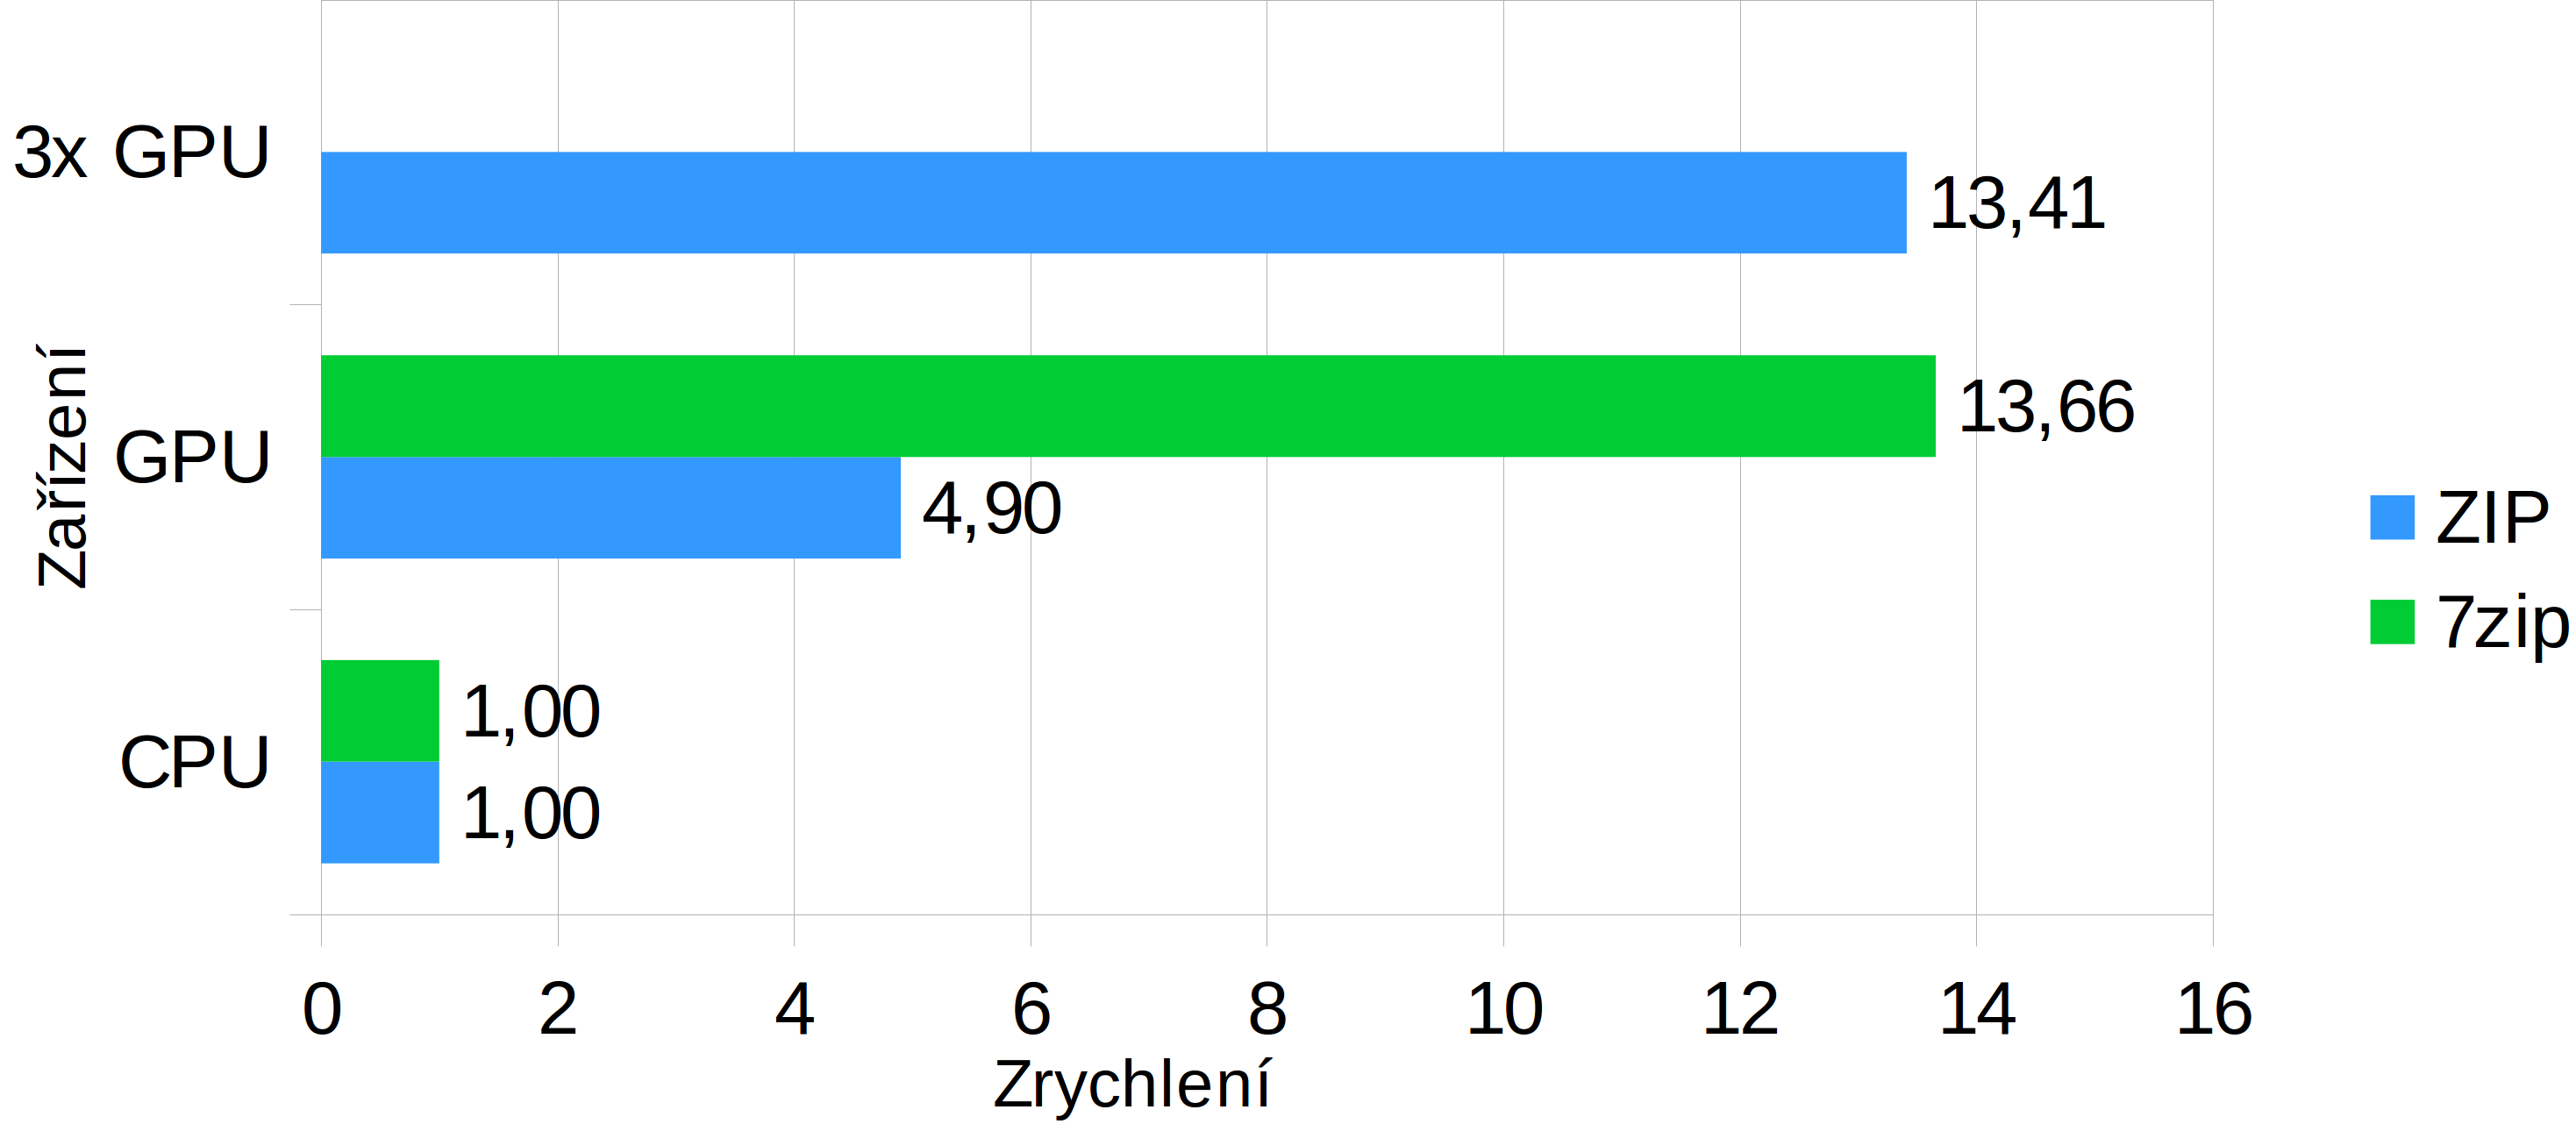
\includegraphics{fig/cpu_gpu_vs_3gpu}
	}
	\caption{Zrychlení obnovy hesel při použití GPU na místo CPU.}
	\label{memory}
    \end{center}
\end{figure}

Očekával jsem, že přidání dalších GPU zvýší celkový výkon alespoň o~80\% což se pro modul ZIP
povedlo překonat. Z~hodnot v~grafu jsem odvodil zrychlení 170\% v~okamžiku, kdy jsem přidal další
2 grafiky.

\begin{figure}[ht]
    \begin{center}
	\scalebox{0.55}{
	    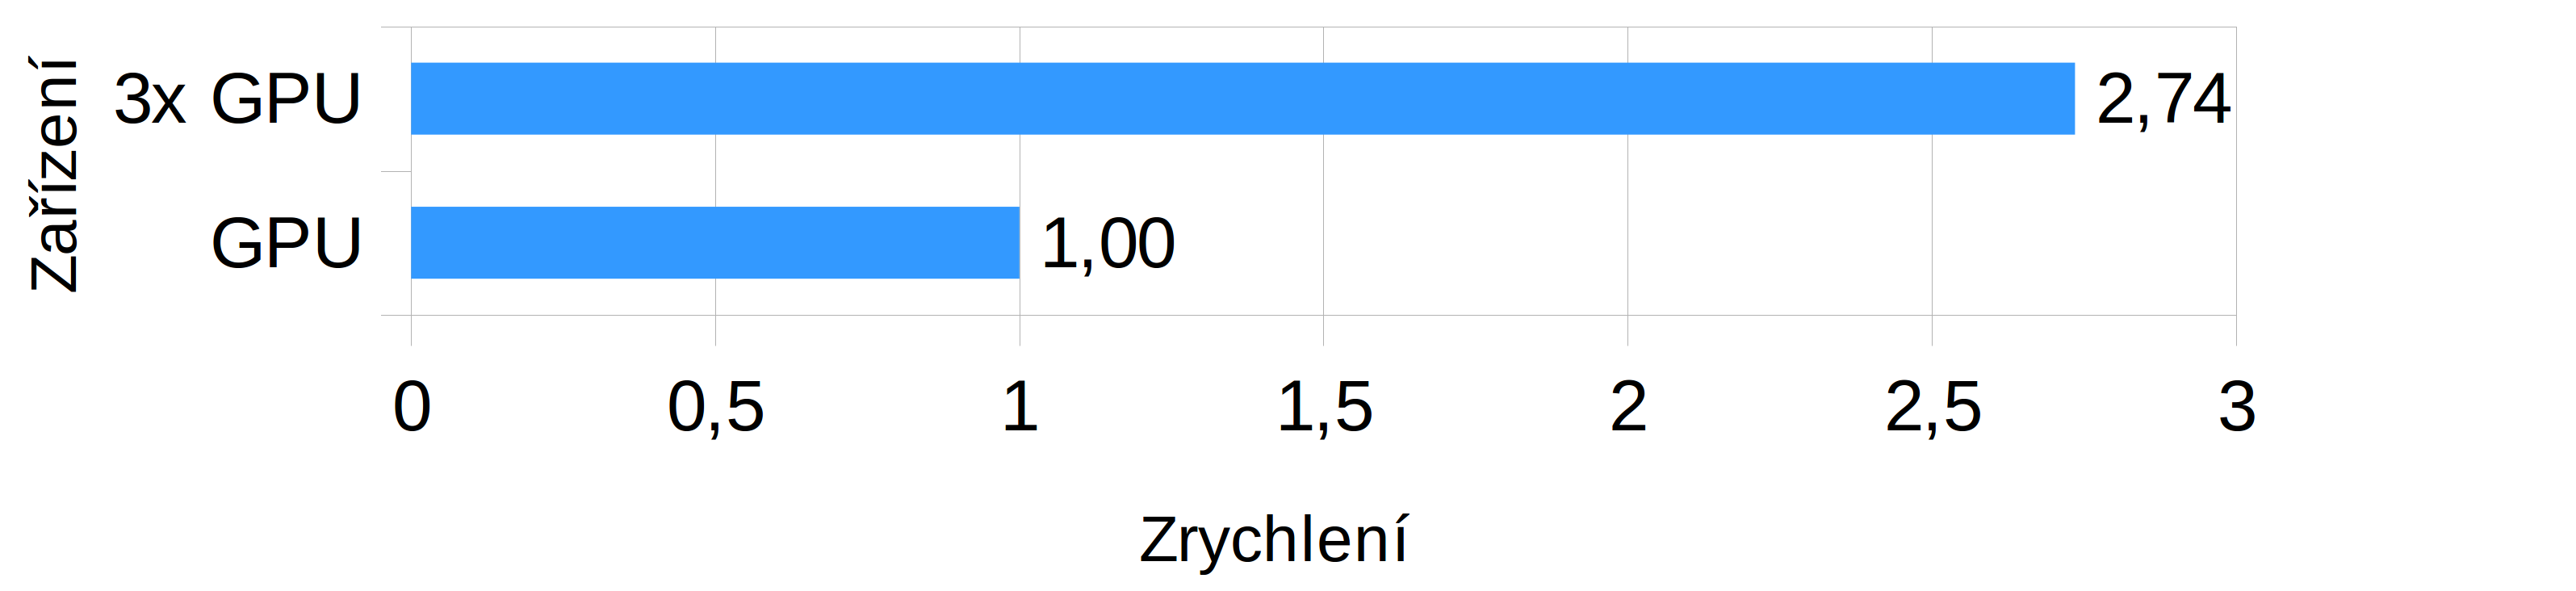
\includegraphics{fig/gpu_vs_3gpu}
	}
	\caption{Zrychlení obnovy hesel při přidání dalších GPU.}
	\label{memory}
    \end{center}
\end{figure}

\chapter{Závěr}
Obsáhnout všechny možnosti a~nastavení analyzovaných formátů je prakticky nemožné z důvodu nízkého
počtu nástrojů schopných tyto hodnoty nastavit, což platí zejména pro formát ZIP.

 Struktury jednotlivých formátů byly popsány tak, aby bylo možné chybějící nebo nejasné informace
dohledat v jejich specifikacích formátu. Jak již bylo zmíněno, struktura 7z souboru je poměrně
komplexní a~proměnná, přičemž bohužel dokumentace tohoto formátu je značně nedostačující. Je tedy
nutné strávit dostatek času studiem struktury formátu, zdrojových kódů a~fóra vývojáře pro získání dalších a~detailnějších informací.

 Výsledky měřeních prokázaly konkurence-schopnost nově přidaných funkcionalit. Z~důvodu
nedostatečných zkušeností s~paralelními aplikacemi a OpenCL nebyly provedeny větší
optimalizace kernelů a zůstává zde tedy prostor pro zvýšení výkonu jednotlivých kernelů. 

 Měření také ukazují, jak silná jednotlivá zabezpečení jsou. Srovnání bezpečnosti šifrování
WinZip AES a metody AES, o jejíž podporu byl Wration rozšířen, nám říká, co bylo pravděpodobně hlavní
důvodem za vytvořením metody WinZip AES. Přidaný AES totiž používá funkce pro generování
šifrovacího klíče, jenž nevyžadují žádné iterace hešovacích funkcí. Tím se toto zabezpečení stává
velmi náchylným k~útokům hrubou silou.

Protějškem k~zabezpečení ZIP pomocí AES je zabezpečení formátu 7zip. Kombinace AES256 a velkého
počtu iterací hešovací funkce SHA256 při generování šifrovacího klíče vede k zabezpečení dat, které
dobře odolává útokům hrubou silou. Pokud použijeme heslo, které se řídí doporučeními pro vytváření
bezpečného hesla, pak lze prohlásit tato metoda zabezpečení, za předpokladu, že nemáme k dispozici
vysoce výkonný superpočítač, za v podstatě neprolomitelnou v reálném čase.

Během práce na nástroji jsem objevil následující možnosti, které by v budoucnu mohly potenciálně
zvýšit výkon modulu 7z v nástroji Wrathion:
\begin{enumerate}
   \item Rozšíření Wrathionu o~možnost zasílání klíčů pro dešifrování z~GPU na CPU. Momentální
       stav je takový, že se klíče generují dvakrát a díky značnému počtu iterací hešovací funkce
       se tímto ztrácí hodně času, než se na CPU vygeneruje klíč znovu.
    \item Další pomůckou pro modul 7z by bylo přidáno využítí více vláken při ověřování hesel na
	CPU. Při současném návrhu modulu GPU slouží pouze jako filtr a CPU ji brzdí, protože musí
	provádět dešifrování a dekompresi dat, aby byl schopen ověřit heslo. GPU je ale schopna
	zaráz označit více hesel jako potenciálně správných. Distribuování ověřování do
	více výpočetních vláken by zrychlilo procházení označených hesel a tím urychlilo
	přirazení nových hesel k~testování.
\end{enumerate}

%=========================================================================

